\documentclass[12pt,oneside]{report}
\usepackage[a4paper]{geometry}
%\usepackage{showkeys}
\usepackage{listings}
\lstset{
language=C,
basicstyle=\tiny\ttfamily}

\usepackage{draftcopy}
\draftcopyName{Joao Paulo}{180}
\usepackage{joaopaulo}
\title{Apostila de Automação Industrial}
\begin{document}

\maketitle
\tableofcontents
\chapter{Sistemas de automação}
%!TEX root = apostila.tex
% \section{Definição}
\label{chap:automacao}
A palavra automação vem do latim \emph{automatus} -- mover por si mesmo. Logo a automação de uma tarefa consiste em fazer com que tal tarefa seja realizada sem envolver trabalho humano. Isto pode ser por diversos motivos: seja por que é uma tarefa perigosa e portanto queremos aumentar a segurança das pessoas, seja para fazer a tarefa de forma mais rápida, seja para melhorar a qualidade do produto final ou seja porque simplesmente o custo do trabalho humano é muito elevado. Logo, podemos definir automação da seguinte forma:
\begin{quote}
  Automação é a substituição do trabalho humano por sistemas autônomos visando melhorar segurança, qualidade, produção e/ou custos.
\end{quote}

Neste contexto, automação industrial é nada mais que a automação de um sistema industrial, ou de um sistema de manufatura. Embora manufatura venha de \emph{fazer com as mãos}, desde a revolução industrial que usamos esta palavra significando simplesmente a fabricação de algum produto. Juntando então o conceito de automação, têm-se:
\begin{quote}
  A automação industrial consiste em implementar os processos necessários para a manufatura de algum produto com o mínimo de esforço humano, físico ou mental, visando melhor segurança, qualidade, produção e/ou custo.
\end{quote}

Com base nesta definição, qualquer sistema que realize a manufatura de algum produto automaticamente e sem usar esforço humano é um sistema automatizado. Logo, uma máquina por mais complexa que seja mas que funcione a manivela, tal como uma calculadora mecânica, não se classifica como automação. Da mesma forma uma máquina que não exija esforço físico mas requeira atenção constante, tal como um carro ou mesmo uma batedeira, também não é automatizada; neste último caso usa-se o termo mecanizada.

Do ponto de vista econômico, a manufatura é a transformação de materiais (matéria prima) em itens de maior valor (produto). Isto é conseguido por uma determinada sequência de processos químicos e físicos. De forma mais sucinta:
\begin{quote}
	Manufatura é a transformação de matéria prima em produtos pela aplicação de um ou mais processos.
\end{quote}

Ou seja, na automação industrial estamos interessados em estudar métodos e ferramentas que permitam deixar os processos de manufatura os mais independentes possível da interferência humana. 

\section{Classificação}

O próprio avanço dos sistemas de automação permite com que se tenham equipamentos cada vez mais versáteis, que não sejam feitos para a fabricação de um único produto. Esta possibilidade de equipamentos versáteis levam a, grosso modo, 3 tipos de automação, tal qual mostra a figura \ref{fig:tipos_automacao}: fixa, flexível e programável. Tipicamente são fatores econômicos que levam a escolha de um destes tipos.

\begin{figure}[hbt]
	\begin{center}
    \includegraphics[width=0.8\textwidth  ]{figuras/fixaflexprog}
%		\includegraphics[width=0.6\textwidth]{tipos_automacao}
	% \tikzstyle{area}=[draw,rectangle,rounded corners,text centered,text width=2.2cm,minimum height=1.2cm]
	% \begin{tikzpicture}
	% 	\draw[very thick, ->, >=stealth'](0,0)--(5.5,0);
	% 	\draw(5.5,0)node[below left]{Diversidade};
	% 	\draw[very thick, ->, >=stealth'](0,0)--(0,3.3);
	% 	\draw(0,3.3)node[above left, rotate=90]{Quantidade};
	% 	\draw(1.25,2.5)node[area]{Fixa} (2.5,1.55)node[area]{Flexível} (4,0.6)node[area]{Programável};
	% \end{tikzpicture}
	\end{center}
	\caption{Tipos de automação industrial quanto a quantidade e diversidade de produtos.}
	\label{fig:tipos_automacao}
\end{figure}

A automação fixa é aplicada à produção de um único produto (ou com mínimas variações), em grandes quantidades: refinaria de petróleo, parafuso, tampas de garrafa, clipes de papel, elos de corrente, biscoito, cerveja, etc. Ela utiliza equipamentos feitos sob medida para cada processo, que portanto tem alto custo inicial mas grande produtividade.

A automação flexível é aplicada à produção de produtos parecidos, em que pequenas modificações permitem a alteração do produto, como por exemplo mudança de um perfil a ser prensado ou extrudado ou a mudança das quantidades do mesmo conjunto de matérias primas (mudança de receita). Tipicamente é feita a chamada fabricação em lotes, onde entre um lote e outro se alteram as peças e/ou as sequências a serem seguidas de forma automática para ter o menor tempo parado possível. Exemplos são livros, circuitos integrados, potes de plástico, panelas, entre outros.

A automação programável é para produção de produtos diferentes mas cujo volume de produção não justifica um processo único. Ela usa máquinas de propósito geral, tais como robôs, ferramentas de controle numérico e impressoras 3d, onde a definição do processo é quase toda feita por \emph{software}, de modo que o custo do maquinário é diluído em diversos produtos.

Estes três tipos não são precisamente definidos, e fica difícil, muitas vezes, determinar que ponto separa uma automação deixa fixa de uma flexível, ou flexível de programável. Por exemplo, uma fábrica de tampas de garrafa PET, que fabrica tampas vermelhas e verdes, em lotes, deixa de ser fixa por conta da mudança da cor?

Mas quanto mais flexível for o sistema de automação, mas necessitado ele é de sistemas de informática e de equipamentos de uso geral controláveis. De modo geral, a automação fixa pode ser realizada a nível de Indústria

A tendência é cada vez mais ter a automação flexível e programável aumentando a capacidade de produção, de modo que a flexível vai ocupando nichos da fixa e a programável da flexível. Apesar disso, em vários casos é difícil imaginar alguns produtos deixando de utilizar a automação fixa.

\section{Pirâmide de automação}

A automação em larga escala de uma grande indústria envolve muito mais que a mera manufatura e inclui problemas de abastecimento, armazenagem, análise de mercado, exigências ambientais, entre várias outras coisas. Uma forma de se separar os diferentes problemas da automação é através da chamada Pirâmide de Automação, mostrada na figura \ref{fig:piramide}.

\begin{figure}[htb]
	\begin{center}
\begin{tikzpicture}[y=0.80pt, x=0.8pt,xscale=0.4,yscale=-0.4, inner sep=0pt, outer sep=0pt]
    \path[fill=black] (530,582.41803) node[above right] (text3018)
      {Instrumentação};
    \path[fill=black] (530,511.83002) node[above right] (text3022) {Controle};
    \path[fill=black] (530,441.0715) node[above right] (text3794)
      {Supervisão};
    \path[fill=black] (530,370.13507) node[above right] (text3798) {Gerência
      de manufatura};
    \path[fill=black] (530,299.51303) node[above right] (text3804)
      {Planejamento estratégico};
      \path[cm={{1.01932,0.0,0.0,1.01932,(-6.1462,-4.25386)}},draw=black,fill=c00ffff,miter
        limit=4.00,line width=2pt] (320.0000,252.3622) -- (423.9230,432.3622) --
        (527.8461,612.3622) -- (320.0000,612.3622) -- (112.1539,612.3622) --
        (216.0770,432.3622) -- cycle;
      \path[cm={{0.80176,0.0,0.0,0.79778,(63.47204,51.63306)}},draw=black,fill=c00ff00,miter
        limit=4.00,line width=2pt] (320.0000,252.3622) -- (423.9230,432.3622) --
        (527.8461,612.3622) -- (320.0000,612.3622) -- (112.1539,612.3622) --
        (216.0770,432.3622) -- cycle;
      \path[cm={{0.60132,0.0,0.0,0.59833,(127.61319,101.96534)}},draw=black,fill=cffff00,miter
        limit=4.00,line width=2pt] (320.0000,252.3622) -- (423.9230,432.3622) --
        (527.8461,612.3622) -- (320.0000,612.3622) -- (112.1539,612.3622) --
        (216.0770,432.3622) -- cycle;
      \path[cm={{0.40088,0.0,0.0,0.39889,(191.75434,152.29762)}},draw=black,fill=cff6600,miter
        limit=4.00,line width=2pt] (320.0000,252.3622) -- (423.9230,432.3622) --
        (527.8461,612.3622) -- (320.0000,612.3622) -- (112.1539,612.3622) --
        (216.0770,432.3622) -- cycle;
      \path[cm={{0.20044,0.0,0.0,0.19944,(255.8955,202.62989)}},draw=black,fill=cff5555,miter
        limit=4.00,line width=2pt] (320.0000,252.3622) -- (423.9230,432.3622) --
        (527.8461,612.3622) -- (320.0000,612.3622) -- (112.1539,612.3622) --
        (216.0770,432.3622) -- cycle;
    \begin{scope}[shift={(3.29592,0)}]
      \path[fill=black] (309.04346,582.41803) node[above right] (text3824) {0};
      \path[fill=black] (310.00049,511.8302) node[above right] (text3828) {1};
      \path[fill=black] (309.28271,441.0715) node[above right] (text3832) {2};
      \path[fill=black] (309.00244,370.13507) node[above right] (text3836) {3};
      \path[fill=black] (309.45361,299.51303) node[above right] (text3840) {4};
    \end{scope}
    \path[fill=black] (79.834969,582.41803) node[above left] (text3858) {Sensores
      eatuadores};
    \path[fill=black] (79.875984,511.8302) node[above left] (text3862) {CLP, SDCD,
      CNC};
    \path[fill=black] (81.256844,441.0715) node[above left] (text3866) {SCADA,
      HMI};
    \path[fill=black] (80.245125,370.13507) node[above left] (text3870) {PIMS, MES,
      LIMS, WMS};
    \path[fill=black] (79.999031,299.51303) node[above left] (text3874) {ERP};

\end{tikzpicture}
	\end{center}
	\caption{Pirâmide de automação.}
	\label{fig:piramide}
\end{figure}

Note que esta não é a única representação da pirâmide: umas começam pelo 1, outras tem apenas 4 camadas, e assim por diante, logo mais importante que o número de cada camada é o que tais camadas significam.

\begin{description}
	\item[Nível 0: Instrumentação] Camada onde se encontram instrumentos, sensores, motores,
máquinas, etc. Consistem nos equipamentos do chamado ``\emph{chão de fábrica}''.
\item[Nível 1: Controle] Controle automático da planta -- onde se localizam os Controladores
Lógico-Programáveis (CLP), os Sistemas Digitais de Controle Distribuído (SDCD), os Controles Numéricos Computadorizados (CNC) e/ou computadores de controle.
\item[Nível 2: Supervisão] Supervisão e controle do processo através de Interfaces Homem-Má
quina (IHMs) ou SCADA (\emph{Supervisory Control And Data Acquisition}).
\item[Nível 3: Gerenciamento da Manufatura] Gestão dos recursos da planta e controle da produção.  Sistemas PIMS
(\emph{Process Information Management System}) e MES (\emph{Manufacturing Execution Systems}).
\item[Nível 4: Planejamento Estratégico] Gestão dos recursos e produção da empresa como um todo. ERP –
\emph{Enterprise Resources Planning}.
\end{description}

A figura \ref{fig:automacao} mostra um diagrama em blocos de um processo automatizado, contendo os blocos representativos dos níveis 0 a 3 da pirâmide de automação. A instrumentação consiste de sensores e atuadores. As variáveis medidas pelos sensores são denominadas de variáveis controladas, enquanto que os valores de comando dos atuadores são chamados de variáveis manipuladas. Como tais atuadores irão operar é definido pelo controle (nível 1), em função de parâmetros definidos pelo supervisório, (nível 2). Este também monitora estas informações e as repassa ao sistema de gerenciamento no nível 3, que aglutina dados de diversos processos para a tomada de decisões de mais alto nível.
\begin{figure}[htb]
	\begin{center}
    \includegraphics[width=0.7\textwidth]{figuras/automacao}
	\end{center}
	\caption{Diagrama em blocos da automação de um processo.}
	\label{fig:automacao}
\end{figure}

Este texto faz um estudo da automação industrial de modo \emph{bottom-up}: começando do nível 0 até o nível 3. O nível 4 é mais importante para um estudo de engenharia de processo ou de produção e portanto não será abordado.

%!TEX root = principal.tex
\chapter{Gerenciamento da manufatura: PIMS e MES}

 PIMS -- \emph{Process Information Management System} e MES -- \emph{Manufacturing Execution System} são sistemas da camada 3 da pirâmide de automação, responsáveis pelo armazenamento e tratamento de dados do nível 2, concentrando os dados de diversos processos separados em um único ponto. São os chamados \emph{middleware}, pois ficam a meio caminho entre os sistemas de gerenciamento de empresa e os supervisórios, às vezes combinando funções de um ou de outro.

 De forma geral, no terceiro nível da pirâmide a preocupação é em consolidar os dados brutos do processo (\emph{data}), para com eles gerar informações  (\emph{information}) e conhecimento (\emph{knowledge}) sobre o processo, aumentando o valor destes valores, como mostra a figura \ref{fig:PIMS_conhecimento1}. Os dados são obtidos ou do controlador ou do supervisório de um determinado processo. A relação entre dados ou a variação destes dados no tempo geram informação sobre a planta. A relação entre informações ou a variação de informações no tempo geram conhecimento.
\begin{figure}[htb]
	\begin{center}
	%	\includegraphics[angle=-90,width=0.8\textwidth]{PIMS_conhecimento1}
		\begin{tikzpicture}[scale=1.5]
		\draw[very thick, ->, >=stealth'](0,0)--(5.5,0);
		\draw(5.5,0)node[below left]{Quantidade de dados};
		\draw[very thick, ->, >=stealth'](0,0)--(0,3.3);
		\draw(0,3.3)node[above left, rotate=90]{Valor};
		\draw[very thick] plot[smooth, tension=1.0] coordinates{(0.2,3.3) (2,1) (5.5,0.3)};
		\draw(0.3,3.)node[right]{Conhecimento} (1.3,1.4)node[above right]{Informação} (4.3,0.4)node[above]{Dados brutos};
	\end{tikzpicture}

	\end{center}
	\caption{Relação entre dados, informações e conhecimentos.}
	\label{fig:PIMS_conhecimento1}
\end{figure}

Um exemplo desta relação é mostrado na figura \ref{fig:PIMS_conhecimento2}. Nesta figura, a partir dos dados de temperatura e vazão de um fluido é gerada a informação do calor removido em determinado trocador de calor. A comparação dos calores removidos de diversos trocadores gera o conhecimento de qual trocador é mais eficiente.

\begin{figure}[htb]
	\begin{center}
		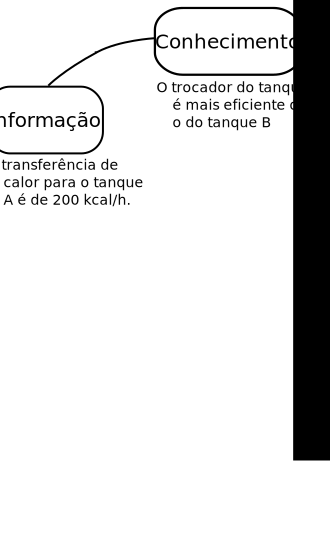
\includegraphics[angle=-90,width=0.8\textwidth]{PIMS_conhecimento2}
	\end{center}
	\caption{Exemplo da transformação de dados para informação e de informação para conhecimento.}
	\label{fig:PIMS_conhecimento2}
\end{figure}

\section{PIMS}
	Para a finalidade de gerar informação e conhecimento, o ponto de partida é obter os dados brutos. Esta é a tarefa principal do PIMS: adquirir, armazenar e apresentar diversos dados de uma planta. O PIMS foi criado e ainda é principalmente usado para processos contínuos, tais como uma refinaria ou siderúrgica, e portanto tem um enfoque muito grande em variáveis analógicas e na relação delas com o tempo.

	Do ponto de vista do PIMS podemos esquematizar os sistemas de uma fábrica como mostra a figura \ref{fig:PIMS}, onde se vê que o PIMS tem 4 partes principais: um
	\begin{description}
		\item[historiador de processos] que se comunica com vários sistemas do nível 1 (CLP, CNC) ou 2 (supervisório) ou ainda de outros sistemas nível 3, tais como um LIMS -- \emph{Laboratory Information Management System} ou MES para obter dados brutos dos diversos processos e acumula-os num
		\item[banco de dados temporal], que armazena os dados indexando-os pelo tempo. Uma
		\item[interface gráfica] faz a recuperação e visualização destes dados, que ainda podem ir para
		\item[aplicações clientes] com variadas funções, desde análise dos dados a interface com outros sistemas.
	\end{description}
	\begin{figure}[hbt]
		\begin{center}
			\includegraphics[angle=-90,width=0.8\textwidth]{PIMS}
		\end{center}
		\caption{Sistema PIMS -- REFAZER.}
		\label{fig:PIMS}
	\end{figure}

\subsection{Historiador de Processos}
O historiador do processo é necessário pelas seguintes funcionalidades:
\begin{description}
 	\item[Registro Histórico] para análise de incidentes, controle de qualidade, métricas de performance, entre outros.
 	\item[Adequação a normas] como por exemplo para controle ambiental.
 	\item[Monitoração de equipamentos] para ontrole de vida útil e apoio à manutenção.
 	\item[Análise de processo], facilitando a visualização de dados e detecção de correlações.
 \end{description}  			

Para tanto o historiador se comunica com sistemas do nível 2 (SCADA) e 1 (CLP) para armazenar os dados do processo. Estes dados são principalmente os valores das variáveis do processo, sejam discretos ou contínuos, mas também abarcam outras informações, tais como a ocorrência de alarmes, a marcação de que operador está presente, o período que um equipamento está ligado, entre outros. Cada uma desta isformações é identificada por um marcador único - a chamada \emph{tag}, ao qual também está associado o endereço lógico de onde se obtém tal informação e o tempo em que tal dado foi gerado (\emph{time stamp}). Em alguns casos se associa também uma métrica da qualidade do dado, referente a confiabilidade daquele dado, tal como se o instrumento de medida está calibrado ou não.

Estas informações podem ser obtidas tanto de sistemas SCADA ou de CLPs. Algumas vantagens de pegar informação dos sistemas nível 2 são que: 
\begin{itemize}
	\item o SCADA já converteu os dados para unidades de engenharia enquanto que em alguns CLPs os dados estão em valor bruto (de 0 a 4095);
	\item muitas variáveis são definidas apenas no sistema SCADA, não existindo nos CLPs, tais como o motivo de alarmes ou qual operador está monitorando a operação;
	\item  interface com os sistemas SCADA costuma ser padrão, o que facilita a comunicação e interoperação.
\end{itemize}

Vantagens de obter as informações do CLP são:
\begin{itemize}
	\item busca dos eventos com menor atraso temporal;
	\item pode-se coletar os dados em um ponto único, se todas as redes de CLPs estiverem interligadas;
	\item CLPs são mais confiáveis e apresentam menor suscetibilidade a falhas que os sistemas SCADA.
\end{itemize}

\subsection{Banco de Dados Temporal}
A maioria das análises realizadas nos dados de um sistema PIMS são em função do tempo, logo é comum ele usar um banco de dados que indexa a informação pelo tempo. Basicamente é uma tabela, relacionando \emph{time stamp}, \emph{tag}, tipo de dado (analógico, booleano, texto), valor e qualidade (se houver).

Um problema do uso deste tipo de banco de dados, ao invés dos chamados bancos de dados relacionais, que são bem mais comuns, é que a busca por informação pode ter uma baixa performance quando a quantidade de dados aumenta muito. Esta é a principal razão para que estes sistemas façam uma compressão de dados, que basicamente se resume a não armazenar dados que não tragam muita informação nova. A figura \ref{fig:reconstrucaoDados} mostra a idéia por trás da compressão de dados.

\begin{figure}[hbt]
	\begin{center}
		\includegraphics[width=0.8\textwidth]{figuras/reconstrucaoDados}
	\end{center}
	\caption{Processo de amostragem, compressão e reconstrução dos dados.} %%TODO:refazer
	\label{fig:reconstrucaoDados}
\end{figure}

Algoritmos comuns para a compressão de dados no PIMS são \emph{banda morta}, onde os dados são apenas armazenados se variarem mais do que um mínimo especificado; o \emph{SDCA -- Swinging Doors Compression Algorithm}, onde para cada valor recebido é definida uma reta entre ele e o último valor armazenado, descartando valores que possam ser definidos por esta reta e mais um erro; e o \emph{boxcar/backslope}, que usa a banda morta e mais uma reta definida pelo último valor armazenado. %%Pequeno. Pode ser expandido

\subsection{Interface Gráfica}
A interface gráfica de um sistema PIMS é, em muitos aspectos, muito parecida com a de um sistema SCADA, contendo representações pictóricas do processo (sinóticos) com os valores de várias variáveis e gráficos de tendência. Tais elementos são melhor vistos no contexto de um sistema SCADA.

\section{MES}
Assim como o PIMS, um sistema MES também adquire dados do processo com o objetivo de apresentar uma visão geral do processo. Porém o MES tem uma função mais ativa que o PIMS, que é focado mais no armazenamento dos dados. Outra diferença importante é que os MES são usados principalmente em processos discretos, muitas vezes em sistemas de automação flexível ou programada, e tem que lidar com o sequenciamento dos processos, o que ocorre menos em sistemas contínuos.

Os sistemas MES agregam diversas funções de sistemas anteriores mais simples e específicos e são definidos por terem 11 funções:
\begin{description}
	\item[Gerenciamento das definições de produto.] Tudo o que é necessário para a fabricação do produto. Isto inclue armazenamento, lista de materiais e insumos, set-points do processo e receitas.

	Por receita, entenda-se uma variação do processo para, na mesma máquina, produzir produtos diferentes ou variações dele. Por exemplo, num processo de pintura a receita diria quais as tintas usadas, em que sequência, em que volume e em que velocidade de aplicação. É muito importante na automação flexível e programável.

	\item[Gerenciamento de insumos.] Permite preparar e executar ordens de produção com garantia de disponibilidade dos insumos.
	\item[Agendamento de produção.] Permite determinar a ordem que a produção será feita, para alcançar os requerimentos de produção definidos pela ERP (camada 4 da pirâmide) utilizando otimamente os recursos.

	Tipicamente inclui ferramentas de simulação, que permitem comparar diversas opções de ordens e estimar efeitos quando de mudanças imprevistas na sequência de produção (tipicamente por conta de uma parada não programada).

	\item[Envio de ordens de produção.] Em função do agendamento feito, o MES cuida de enviar as ordens de produção para os diversos postos da planta.
	\item[Acompanhamento da execução de ordens de produção.] Comunicação com sistemas níveis 1 e 2 para garantir a execução das ordens. Inclui também o registro de paradas.

	O registro de paradas é feito automaticamente quando o equipamento para, seja por alguma condição espúria detectada no nível 1 ou por ação do operador no nível 2. Em ambos os casos fica registrado uma parada em aberto, que só finaliza quando o operador complementar certas informações que auxiliam no diagnóstico da parada e o equipamento voltar a funcionar.

	\item[Coleção dos dados de produção.] Equivalente ao historiador de processo do PIMS.
	\item[Análise da performance da produção.] Cálculo dos chamados índices de produção -- \emph{KPI, Key Performance Indicators}. É a geração de informação útil a partir dos dados da produção.

	Como exmplo de um KPI, temos o OEE -- \emph{Overall Equipment Effectiveness} -- que aponta a efetividade de um determinado equipamento ou célula de produção. Este índice é dado por:

\begin{equation}
	\text{OEE} = \text{disponibilidade}\times\text{performance}\times\text{qualidade,}
\end{equation}
onde por disponibilidade entende-se a razão entre o quanto de tempo o equipamento funcionou e o quanto de tempo ele deveria ter funcionado, ou seja, descontando-se as paradas não programadas; performance é a razão entre a produção do equipamento enquanto funcionava e a capacidade de produção de que o equipamento é capaz, ou seja, descontando a ociosidade do equipamento; e qualidade é o valor do que o equipamento produziu em relação ao valor se não tivesse havido nenhum descarte ou geração de produtos de menor valor.

	\item[Rastreamento da produção.] Permite levantar que produto ou lote foi feito quando e em qual equipamento. Útil para melhoria da produção e imprescindível para remédios e produtos alimentícios.
	\item[Armazenamento dos logs de produção.] Hoje em dia tais logs são inseridos pelo operador no próprio sistema supervisório e realcionados às variáveis de produção.
	\item[Interface de auditoria.] Permite a análise dos diversos dados e informações armazenados e o cruzamento destes dados com outras bases de dados.
\end{description}
\section{Gerenciamento da manufatura: MES}
%!TEX root = apostila.tex
Na pirâmide de automação, a partir da camada 2, os sistemas utilizados são softwares em computadores, sejam servidores, terminais, desktops, notebooks ou mesmo tablets e smartphones (para o caso do supervisório). No nível de controle, o dispositivo utilizado pode ser um computador, um CLP -- que não deixa de ser um computador -- ou outro dispositivo que incorpora um processador. Hoje em dia até no nível 0 estão ficando cada vez mais comuns os dispositivos ditos \emph{inteligentes}, que incorporam também um microprocessador.

Tais dispositivos digitais abrem espaço para que a comunicação entre eles seja através de um sinal digital, com vantagens em relação a sinais analógicos em imunidade a ruído, possibilidade de redução de custos e de aumento da quantidade de informação, maior facilidade de aplicação de criptografia, entre outras.

Deste modo se conectam os diferentes dispositivos que fazem parte de um sistema de automação através de uma rede de comunicação, de onde vem a importância de entendê-las e estudá-las.

\section{Redes de Comunicação: Introdução e noções básicas}

O problema da comunicação de dados automática entre diversos dispositivos é bastante complexo. Peguemos como exemplo pagar uma conta via internet: é necessária a comunicação do dispositivo caseiro (que seja um tablet) e o computador central do banco (1). Quanto mais rápida for esta comunicação, mais agradável é para o usuário e mais barato é para o usuário e para o banco (2). Obviamente nenhuma das partes envolvidas querem que seja pago o valor errado ou a conta errada (3). Entre o tablet e o servidor do banco estão: o modem wifi, a central telefônica, servidores da companhia telefônica e talvez de outras fornecedoras de serviço (4), e em geral não é do interesse do usuário que a companhia telefônica ou outro elemento saiba de sua senha do banco (5). A comunicação do tablet ao modem é por wifi. Do modem para a central telefônica é pelo fio telefônico. Da central em diante pode ser por cabos de cobre ou, mais provavelmente, por fibra óptica (6). Também, por questão de custos e privacidade, não é desejável que outros elementos recebam aquela informação, mesmo que criptografada (7).

Ou seja, podemos definir, extendendo ao caso geral, que a comunicação de dados envolve:
\begin{enumerate}
	\item transferência de dados de um dispositivo a outro,
	\item em alta velocidade,
	\item sem perda de informação,
	\item passando por dispositivos intermediários,
	\item com privacidade,
	\item envolvendo meios e sistemas de comunicação diferentes,
	\item sem envolver outros dispositivos desnecessariamente.
\end{enumerate}

Claro que há vários casos que não envolvam todos estes aspectos. Pode-se ter comunicações digitais bem mais simples, como no caso de um mouse "conversando" com o computador através da USB, que não requer alta velocidade, nem tem dispositivos intermediários, logo a princípio não requer privacidade nem diferentes meios de comunicação e nem é possível de envolver outros dispositivos. Até mesmo a questão da perda de informação pode não ser necessária em alguns casos, tais como em sistemas VOIP (\emph{Voice Over IP}), onde mais importante que garantir que todos os dados tenham sido recebidos corretamente é manter o atraso da comunicação pequeno o suficiente para não incomodar demais. Mas consideremos inicialmente o caso mais geral.

Para resolver um problema de tal magnitude, foi desenvolvida a idéia de quebrá-lo em várias partes, ou camadas, onde cada camada tem um protocolo responsável por uma determinada parte do problema. A informação fica então passando de camada a camada, acrescida de metadados para resolver todas as questões relativas à comunicação. Tal esquema é também chamado de pilha de protocolos. O chamado modelo OSI foi então criado definindo camadas o mais genéricas possíveis, de modo a abarcar qualquer tipo de comunicação de dados.

\subsection{Modelo OSI}
O modelo OSI (\emph{Open System Interconnection}) é o modelo de referência de redes de dados, criado em 1970 e adotado pela ISO em 1983. Este modelo define 7 camadas de abstração que separam as diferentes tarefas necessárias à comunicação de dados; são as camadas: física, enlace, rede, transporte, sessão, apresentação e aplicação.

\subsubsection{Camada 1 -- Física}
	A camada física é a única que não pode ser implementada em software. Ela lida com as definições eletro-mecânicas necessárias para a comunicação. Ou seja, a camada física define:
	\begin{itemize}
		\item o meio pelo qual os dados são transmitidos -- sinais elétricos por cabo, sinais de rádio, luz, etc;
		\item as características do meio de transmissão, tais como o tipo de cabo, os níveis de tensão, o formato dos conectores, etc;
		\item a taxa de transmissão (tipicamente quantos bits por segundo -- bps).
	\end{itemize}
	Note-se que a taxa de transmissão acaba sendo limitada justamente pelos diversos parâmetros físicos descritos pela camada física de um determinado protocolo de comunicação.

Outro parâmetro definido na camada física é se a rede é \emph{simplex}, \emph{half-duplex} ou \emph{full-duplex}. Simplex significa que a comunicação no meio de transmissão é apenas num sentido (exemplo: televisão), half-duplex é uma comunicação em dois sentidos, mas apenas um por vez (exemplo: walkie-talkie) e full-duplex é uma comunicação em ambos os sentidos ao mesmo tempo (exemplo: telefonia).

A camada física também limita aspectos da chamada topologia da rede, que é a forma como os dispositivos se relacionam entre si, como por exemplo:
\begin{description}
	\item[Ponto-a-ponto] Onde apenas 2 dispositivos se conectam ente si.
	\item[Estrela] Onde um nó central se comunica com os demais nós. Vide sistemas de TV ou rádio.
	\item[Barramento] Onde os vários dispositivos se conectam em paralelo a um único barramento.
	\item[Árvore] Um barramento com derivações.
	\item[Linha] Onde cada dispositivo se conecta diretamente apenas com um ou 2 vizinhos.
	\item[Anel] Uma linha formando um anel.
	\item[Totalmente conectada] Cada dispositivo diretamente conectado a todos os outros da rede.
	\item[Malha] Cada nó conectado a vários outros, sem uma hierarquia ou ordem bem definida.
\end{description}

\subsubsection{Enlace}

A camada de enlace cuida da comunicação de um dispositivo a seu vizinho, que não necessariamente são os pontos inicial e final de uma comunicação.

No exemplo dado acima, do pagamento de conta na internet, esta camada cuida da comunicação entre o tablet e o modem wifi; entre o modem e a central; entre a central e o servidor da companhia telefônica, e assim por diante.

A camada de enlace de um protocolo define:
\begin{itemize}
	\item quem acessa o meio de transmissão e quando,
	\item que sinais indicam o início e o fim de uma transmissão,
	\item mecanismos que detectem e/ou corrijam erros e,
	\item se necessário, para qual dentre vários dispositivos é aquela comunicação específica.
\end{itemize} 

Alguns protocolos de comunicação, tais como USB e ethernet, fazem a conexão ponto a ponto. Neste caso apenas 2 dipositivos podem acessar o meio. Outros sistemas, como o wifi, podem ter vários (em alguns casos, centenas) de dispositivos no mesmo meio. O que torna necessário a definição de quem pode acessar o meio em cada instante. Várias possibilidades existem, entre as quais:
\begin{description}
	\item[mestre-escravo] Neste sistema, a comunicação sempre é iniciada pelo mestre, e um escravo só ocupa o meio quando o mestre requisita uma informação. Ex.: USB, Modbus.
	\item[\emph{token ring}] É passada uma ficha (\emph{token}) virtual entre os dispositivos. Quem tem a ficha pode falar.
	\item[Multiplexação por tempo] Cada dispositivo tem uma hora específica para controlar o barramento. Um sinal periódico (NUT- \emph{Network Update Time}) sincroniza os dispositivos.
	\item[CSMA-CD -- \emph{Carrier Sense Multiple Access with Collision Detection}] Sempre que um dispositivo quer se comunicar com outro, ele checa antes se o meio está livre. Ex.: wi-fi, bluetooth, CAN.
\end{description}

Tipicamente os protocolos da camada de enlace acrescentam uma certa redundância ao dado transmitido, o que permite detectar e até corrigir erros de transmissão. São os chamados códigos corretores de erro, dentre os quais se utiliza bastante o CRC - \emph{Cyclic Redundancy Check}, mas outros são possíveis, desde uma simples checagem de paridade (se há um número ímpar ou par de bits com valor 1), usado nos protocolos de comunicação serial RS232, RS422 e RS485, a códigos convolucionais, usados na ethernet e em redes celulares.

\subsubsection{Rede}
Camada responsável pelo roteamento da informação. Ou seja: Se A quer se comunicar com D, mas A apenas tem ligação direta com B e C, para quem A deve mandar a informação?

Tipicamente este roteamento é feito através de uma tabela que mapeia o endereço lógico de um dispositivo (o endereço usado nas etapas acima, tais como o IP) e o endereço físico, usado pela camada de enlace. Muitos sistemas usam o \emph{MAC address} -- \emph{Medium Access Control Address}, que é um código definido no dispositivo quando de sua fabricação, tipicamente de 48 ou 64 bits, e único para cada dispositivo.

Esta é a última camada a que uma comunicação chega num dispositivo que não o inicial ou final: o programa desta camada checa se o endereço lógico da mensagem é o mesmo daquele dispositivo. Caso contrário, ele busca na tabela de roteamento qual o endereço físico para o qual reenviar aquela mensagem e reenvia, eventualmente através de um dispositivo diferente ou com um protocolo diferente, tal qual mostra a figura \ref{fig:camada_rede}. Isto serve também para fazer a conexão entre diferentes redes.

\begin{figure}[hbt]
	\begin{center}
		\includegraphics[width=0.6\textwidth]{figuras/network_layer}
	\end{center}
	\caption{Comunicação passando por dispositivo intermediário.}
	\label{fig:camada_rede}
\end{figure}

\subsubsection{Transporte}
 A camada de transporte cuida da comunicação entre o ponto inicial e final.

 São responsabilidades desta camada:
 \begin{itemize}
	 \item garantir a confiabilidade da transmissão, checando se determinado pacote chegou ou não ao destino,
	 \item controlar o fluxo de dados na rede, impedindo de mandar dados de mais que ou sejam mais que o receptor aguente ou que congestionem a rede.
 \end{itemize}
 
 Para melhor ajustar o fluxo de dados, esta camada pode resolver quebrar uma mensagem grande em vários pacotes, mandando um pacote de cada vez para a camada de rede e remontando a mensagem no recebimento. Este é o procedimento usado na transmissão de dados na internet.

 Um conceito interessante utilizado na camada de transporte é o de \emph{Quality of Service -- QoS}, qualidade de serviço. Embora não seja um número único, mas sim a definição de vários parâmetros de uma rede, tais como a ordem de chegada dos pacotes, o atraso na entrega e a falha da entrega de pacotes, a grosso modo pode-se dizer que um alto QoS garante a chegada de todos os pacotes, na ordem em que foram enviados.

 A internet foi originalmente pensada como um sistema de baixo QoS, voltado para a trasnmissão de arquivos. A ordem dos pacotes, a princípio, não interessava e nem o atraso de um pacote. Caso um pacote se perca, simplesmente pede-se que seja reenviado. Uma rede de telefonia, por outro lado, busca garantir que o tempo de cada pacote seja o mesmo, para não piorar a qualidade da voz transmitida.

 Para diversas aplicações industriais, o QoS é importante: não se pode aceitar que uma mensagem de alarme, por exemplo, demore muito a chegar. EtherCAT - \emph{Ethernet for Control Automation Technology} é um exemplo de uma modificação do protocolo Ethernet para mensagens com diferentes QoS.
 
\subsubsection{Sessão}
Esta camada cria, gerencia e termina conexões entre 2 pontos de uma rede. É mais comum na telefonia, onde se gera um caminho fixo para uma determinada ligação. Quando implementada, esta camada gera a tabela que é usada pela camada de rede.

\subsubsection{Apresentação}
Faz a mudança no formato dos dados. Exemplo: troca de quebra de linha entre sistemas Unix e Windows, mudança de codificação windows 1252 para UTF, etc.

Inclue também a criptografia, que é a base para garantir a privaciade da comunicação ponto-a-ponto.

\subsubsection{Aplicação}
A aplicação final, que gera e/ou consome o dado transmitido.

\subsection{Internet}
	A Internet define uma pilha de apenas 4 protocolos: \textbf{enlace}, que engloba também o físico e para o qual há várias possibilidades, tais qual Ethernet, usando par trançado, 802.11, para wi-fi, FC (\emph{Fibre Channel}) 8b/10b para conexões de fibra óptica, entre outros; \textbf{IP} -- \emph{Internet Protocol}, equivalente ao de rede do modelo OSI; \textbf{transporte}, que pode ser um entre vários, sendo o TCP e o UDP os mais comuns e o de aplicação, que envolve sessão, apresentação e aplicação num só, e para o qual existem inúmeros
	.

	A figura \ref{fig:tcp-ip} mostra a sequência que é feita com uma informação passada por http pela internet.
	\begin{figure}[hbt]
		\begin{center}
			\includegraphics[width=\textwidth]{figuras/tcp-ip}
		\end{center}
		\caption{Encapsulamento da informação na pilha TCP/IP}
		\label{fig:tcp-ip}
	\end{figure}

Como exemplo, um navegador de internet tem vários protocolos do nível de aplicação: http, para buscar páginas não criptografadas, https, para páginas criptografadas, dns, para descobrir o endereço ip relacionado a um determinado endereço, entre outros.

Ao se abrir uma página, tal como a pudim.com.br, o computador primeiramente pega o endereço digitado (\emph{www.pudim.com.br}) e manda uma mensagem ao servidor de dns, que normalmente é definido pelo provedor de acesso, requisitando o endereço IP relativo a este endereço, que no caso é \emph{54.207.20.104}. Ao retornar o endereço, o navegador agora manda uma mensagem tipo \emph{get} pelo protocolo \emph{http} ao IP indicadao pelo servidor DNS e espera um resposta de código 200 do servidor do google, indicando que o que foi pedido existe e contendo a informação pedida, que no caso é o código html da página principal do site.

Este código contém referência a dois arquivos: um arquivo de formatação \verb|estilo.css| e outro de imagem \verb|pudim.jpg|. Cada arquivo deste deve ser pedido por um comando \emph{get} separado.

Toda comunicação neste protocolo é feita usando o protocolo de transporte TCP, que manda cada pacote e espera uma resposta do outro lado. Caso o outro lado não responda ou responda dizendo que teve erro no transporte, o TCP cuida de mandar de novo o pacote para garantir o recebimento do outro lado.

E cada pacote TCP enviado segue pelo protocolo IP (\emph{Internet Protocol}), que pega o endereço IP e através da tabela de roteamento identifica por qual dispositivo de rede (se houver mais de um) e para qual endereço MAC deve mandar aquela informação.
\chapter{SCADA -- Supervisory Control and Data Acquisition}
\section{Arquitetura de sistemas SCADA e interfaceamento com níveis de automação}
\section{Funcionalidades principais de sistemas SCADA}
%!TEX root = principal.tex
\chapter{Sistema SCADA MANGO}
Mango é uma solução SCADA/HMI open source que roda em um sevidor internet java. Logo toda interface dele é através de um navegador. Muito embora ele seja open source, existem versões aprimoradas dele que apresentam umas facilidades a mais, mas a versão básica já permite fazer um sistema SCADA completo.

\section{Instalação}
Vide \emph{http://infiniteautomation.com/wiki/wiki.php}, a instalação é simplesmente descompactar um arquivo zip e rodar um script para abrir o programa. Basta ter o java 1.7 instalado.

\section{Uso}
Ao rodar o mago, ele abre a tela mostrada na figura \ref{fig:mango_login}. A página do mango pode ser acessada novamente pelo endereço \emph{http://localhost:8080}. O login padrão é \textbf{admin}, senha \textbf{admin}.
\begin{figure}[hbt]
	\begin{center}
		\includegraphics[width=\textwidth]{figuras/mango_login}
	\end{center}
	\caption{Tela de login do mango.}
	\label{fig:mango_login}
\end{figure}

O topo da tela do mango pode ser visto na figura \ref{fig:mango_topo}. Na parte mais superior tem os indicadores de eventos e alarmes, seguido dos links para as diversas áreas do mango.
\begin{figure}[hbt]
	\begin{center}
		\includegraphics[width=\textwidth]{figuras/mango_topo}
	\end{center}
	\caption{Topo da tela do mango.}
	\label{fig:mango_topo}
\end{figure}

Um dos primeiros pontos a ser definido é o das fontes de dados do sistema. Chega-se nisto clicando no ícone \emph{data sources}, vide figura \ref{fig:mango_sources}. São possíveis diversos tipos diferentes de fontes de dados, mas para nós no momento os que vão interessar são o \textbf{Modbus I/P}, o \textbf{Modbus Serial} e o \textbf{Virtual Data Source}, este último principalmente para simulação.
\begin{figure}[hbt]
	\begin{center}
		\includegraphics[width=\textwidth]{figuras/mango_sources}
	\end{center}
	\caption{Tela de fontes de dados.}
	\label{fig:mango_sources}
\end{figure}

Para cada fonte de dados, são criados pontos (\emph{data points}), correspondentes a uma tag. No caso de uma fonte virtual, há opções quanto ao tipo de dado (binário, multi-estado, numérico, texto) e quanto ao valor automático, vide figura \ref{fig:mango_virtual}.
\begin{figure}[hbt]
	\begin{center}
		\includegraphics[width=\textwidth]{figuras/mango_virtual}
	\end{center}
	\caption{Definição de dados virtuais para simulação.}
	\label{fig:mango_virtual}
\end{figure}

O protocolo modbus é um dos utilizados na automação industrial. Existe uma implementação do modbus serial para arduino, que é implementado pelo uso da biblioteca \textbf{SimpleModbusSlave}, que faz o arduino trabalhar como um escravo modbus. O data source Modbus Serial nos permite então obter dados de um arduino, seguindo este protocolo.

A configuração do Modbus para a comunicação com o arduino é tal como mostrado na figura \ref{fig:mango_modbus}. É importante que a porta seja a mesma do arduino, bem como bit rate (baud rate), data bits, stop bits, stop bits e parity. O encoding deve ser do tipo RTU e deve se marcar a caixa \textbf{Contiguous batches only}.

\begin{figure}[hbt]
	\begin{center}
		\includegraphics[width=\textwidth]{figuras/mango_modbus}
	\end{center}
	\caption{Definição de uma fonte de dados do tipo modbus serial.}
	\label{fig:mango_modbus}
\end{figure}

O modbus trabalha endereçando o escravo pelo \emph{slave id}, que no caso usamos 1. Os dados são armazenados nos chamados registradores (\emph{registers}). Enquanto o Modbus especifica 4 tipos de registradores, o arduino implementa apenas o \emph{Holding register}, logo nossos pontos devem ser todos deste tipo e concordar com a sequencia definida no arduino.
Cada registrador é de 16 bits. Podemos definir um ponto binário como sendo um único bit daquele registrador ou um ponto numérico, que usa todos os 16 bits.

\section{\emph{Watch list}}
Podemos observar o comportamento dos pontos criados na tela \emph{Watch lists} (figura \ref{fig:mango_watch}). Se o ponto for configurável (settable), também podemos fazé-lo por esta tela.

\begin{figure}[hbt]
	\begin{center}
		\includegraphics[width=\textwidth]{figuras/mango_watch}
	\end{center}
	\caption{\emph{Watch lists} para observar as variáveis.}
	\label{fig:mango_watch}
\end{figure}

\section{Tela gráfica}
A interface normal com o operador é feita através do sinótico -- a representação gráfica do processo. O mango permite montar uma tela gráfica apresentando os diversos valores das variáveis e os controles, como mostra a figura \ref{fig:mango_tela}. A apresentação de variáveis é de forma bem direta, através dos diversos comandos de gif analógico, gif binário, gif dinâmico e gráficos. O ajuste de valores, porém, é um pouco mais complexo.
\begin{figure}[hbt]
	\begin{center}
		\includegraphics[width=\textwidth]{figuras/mango_tela}
	\end{center}
	\caption{Montagem de sinótico.}
	\label{fig:mango_tela}
\end{figure}

Pode-se ajustar o valor de um ponto no mango marcando a opção \textbf{Exibir controles}, a partir do que se pode abrir uma caixinha que permite a escrita do valor na variável. Esta opção porém é mutio pouco prática.

Outra opção mais interessante é através dos \emph{server side scripts}, ou scrpts do servidor. Nestes casos define-se um comando em javascript que permite ler e alterar o valor de uma variável. A página \textbf{http://infiniteautomation.com/wiki/doku.php?id=graphics:mango\_graphic\_views:server\_side\_script\_examples} mostra vários exemplos de códigos úteis para esta tarefa. 

Um adendo: os códigos da página supracitada consideram os endereços a partir da pasta \textbf{<mango>/web}. Porém o arquivo zipado do Mango não contém aí a subpasta Graphics, o que faz com que os exemplos não funcionem. é necessário copiar a pasta \textbf{<mango>/web/modules/sstGraphics/web/graphics} para este local. Pode-se (e deve-se) acrescentar outras imagens mais interessantes a este diretório.
\chapter{Controladores Lógico-Programáveis (CLP)}
%!TEX root = principal.tex
\chapter{Programação - arduino}

Como na parte de processamento de um CLP fica um microcontrolador, faz sentido estudar um pouco este elemento para entender a programação de um CLP mais para a frente. Hoje em dia a plataforma mais comum de microcontrolador é o arduino, portanto foi escolhido para exemplificar esta tarefa.

O arduino é uma plataforma de microcontrolador simplificada para permitir facilidade de uso. O nome arduino refere-se a: uma placa com um microcontrolador Atmel, uma linguagem de programação e um ambiente de desenvolvimento para esta linguagem. E também um antigo auto-proclamado rei da Itália, mas este último não importa para nós.

A placa Arduino tem um conector USB para se ligar ao computador. Isto serve tanto para programar o microcontrolador quanto para comunicação entre os 2. Existem várias versões do arduino, pois já que é um sistema \emph{open-source}, quem quiser pode fazer sua versão diferente da placa. Vamos nos referenciar aos arduinos UNO ou outras placas compatíveis com ele.

O arduino UNO tem 4 barras de pinos fêmeas para conexão com outros dispositivos: uma com tensões de alimentação (\bfseries{POWER}), um com 6 entradas analógicas (\bfseries{ANALOG IN}) e 2 com um total de 14 entradas e saídas digitais (\bfseries{DIGITAL}).
\begin{figure}[hbt]
	\centering
	\includegraphics[width=\textwidth]{figuras/Arduino-Uno-Pinout}
	\caption{Pinagem do Arduino Uno}
	\label{fig:pinagem-arduino-uno}
\end{figure}

A linguagem de programação arduino é basicamente a linguagem C++ para microcontroladores ATMEL, mas com algumas funções e definições facilitadoras. A principal diferença entre C++ e a linguagem arduino é que não existe a função main(), mas sim as funções (ou rotinas) \lstinline|setup()| e \lstinline|loop()|. A função \lstinline|setup()| é executada apenas uma vez no momento que o arduino é ligado (ou resetado) e depois o código dentro da função \lstinline|loop()| é executado repetidamente. Com isto o esqueleto de um programa arduino fica:

\begin{lstlisting}[caption=Esqueleto de um programa arduino., label=lst:ardEsquel]
void setup() {
  //codigo a ser executado no inicio
}

void loop() {
  //codigo a ser executado repetidamente
}
 \end{lstlisting}

Lembrando que no arduino, como no C, tudo que tiver depois de \lstinline|//| é comentário e é ignorado pelo compilador.

\section{Piscando um led.}
Vamos passar logo a um exemplo para analisar um programa arduino. As placas de arduino UNO já tem um led ligado ao pino 13, identificado por um \bfseries{L} na placa. Podemos fazer um programa que faça este led piscar.

\begin{lstlisting}[caption= Programa para piscar led.,label=lst:piscaled]
void setup() {
  //codigo a ser executado no inicio
  pinMode(13,OUTPUT); //define o pino 13 como uma saida (led)
}

void loop() {
  //codigo a ser executado repetidamente
  digitalWrite(13,LOW);  //apaga o led
  delay(500);            //espera meio segundo
  digitalWrite(13,HIGH); //acende o led
  delay(500);            //espera meio segundo
}	
\end{lstlisting}

A chamada \lstinline|pinMode(13, OUTPUT);| serve para definir que o pino 13 será uma saída. Obviamente isto só precisa ser feito no início do programa, logo está dentro de \lstinline|setup()|. Se quiséssemos ter uma entrada digital, usaríamos a mesma função, mas trocando OUTPUT por INPUT: \lstinline|pinMode(pino,INPUT);|.

A função que define o valor de um pino digital é a \lstinline|digitalWrite(pino,valor)|. Ela é chamada duas vezes no código \ref{lst:piscaled} dentro de \lstinline|loop()|, uma para apagar o led (gravando \lstinline|LOW|) e outra para acendê-lo (gravando \lstinline|HIGH|). \lstinline|LOW| e \lstinline|HIGH| são duas constantes, de valor 0 e 1, referentes ao zero e um lógico, respectivamente. Em termos físicos, no sistema arduino o \lstinline|LOW| é uma tensão próxima a \SI{0}{V} e o \lstinline|HIGH| uma tensão próxima a \SI{5}{V}.

Um detalhe é que o microcontrolador do arduino funciona numa velocidade de 8 ou \SI{16}{MHz} (dependendo da versão), logo se colocássemos apenas as duas chamadas à função \lstinline|digitalWrite| não veríamos o led piscar, mas teríamos a impressão que ele está aceso com metade da intensidade. Para vermos o led piscar é necessário colocar um atraso, que é justamente obtido pela função \lstinline|delay(x)|, que gera um tempo morto de \lstinline|x| milisegundos.

Se quiséssemos saber o valor de um pino digital que tivesse sido definido como entrada, a função seria \lstinline|digitalRead(pino)|, que retornaria o valor digital naquele pino. Pode-se usar isto por exemplo, para fazer com que uma saída digital seja a cópia de uma entrada digital, como no código \ref{lst:ardCopiaDig}.
\begin{lstlisting}[caption= Programa para acender um led em função de uma entrada digital.,label=lst:ardCopiaDig]
const int pinoSaida = 13;
const int pinoEntrada = 10;

int valor;

void setup() {
  //codigo a ser executado no inicio
  pinMode(pinoSaida,OUTPUT); //define a saida (led)
  pinMode(pinoEntrada,INPUT); //define a entrada
}

void loop() {
  //codigo a ser executado repetidamente
  valor = digitalRead(pinoEntrada); //le a entrada
  digitalWrite(pinoSaida,valor);  //e escreve na saida
}	
\end{lstlisting}

No código \ref{lst:ardCopiaDig} acrescentamos também algumas variáveis. Duas são constantes com os pinos usados. Elas facilitam a leitura do código e também facilitam caso posteriormente quisermos mudar os pinos utilizados. A outra variável armazena o valor lido da entrada, que depois é escrito na saída. 

%Altere o código do seu programa para que ele faça piscar um led ligado ao pino 5 do arduino.
\section{Sinais analógicos}
Em contraste com os sinais digitais, os sinais analógicos são aqueles que podem assumir qualquer valor de tensão. No contexto do arduino, os sinais analógicos estão limitados a valores entre \SI{0}{V} e \SI{5}{V} em relação ao terra.

Para valores analógicos, usamos as funções \lstinline|analogWrite(pino,valor)| e \lstinline|analogRead(pino)|, que, ao contrário das equivalentes digitais, são restritas a alguns pinos específicos. As entradas analógicas são identificadas pelos pinos ANALOG IN (A0 a A5 no arduino) e são ligadas a um conversor analógico/digital (A/D) do microcontrolador, que transforma estes sinais numa palavra binária de 10 bits. Como $2^{10} = 1024$, isto significa que a função \lstinline|analogRead| retorna um valor entre 0 (para uma entrada de 0 V) e 1023 (para uma entrada de 5 V).

Há ainda a função \lstinline|analogWrite|, que gera valores ``analógicos''. Na verdade, o arduino, como a maioria dos microcontroladores, não tem um conversor D/A, logo a função \lstinline|analogWrite| não gera um sinal analógico verdadeiro no pino. O que esta função faz é gerar um sinal modulado por largura de pulso - PWM (\emph{Pulse Width Modulation}).

O sinal PWM é um trem de pulsos digital, com frequência da ordem de \SI{500}{Hz} (no caso do arduino) cuja razão entre o tempo em alto e o perído (conhecida como \emph{duty cycle}) pode ser alterada pelo parâmetro passado, como mostra a figura \ref{fig:pwm}.
\begin{figure}[hbt]
	\centering
	\includegraphics[width=\textwidth]{figuras/pwm}
	\caption{Reta modulada em largura de pulso (PWM).}
	\label{fig:pwm}
\end{figure}	
 Se um sinal PWM é enviado a um pino com um led, ele piscará 500 vezes por segundo, o que é muito rápido para o olho humano, de modo que na prática o que se vê quando se varia o duty cycle de um sinal PWM que aciona um led é uma variação de sua intensidade. Logo um sinal PWM funciona, para muitas aplicações, como um sinal analógico.

Tal como apenas alguns pinos tem a capacidade de ler sinais analógicos, também não são todos os pinos do arduino que conseguem gerar um sinal PWM, logo a função \lstinline|analogWrite| está restrita aos pinos 3, 5, 6, 9, 10 e 11 (do arduino UNO. Outros podem usar outros pinos). Um outro detalhe que vale a pena ressaltar é que enquanto a função \lstinline|analogRead| gera um valor entre 0  1023, a \lstinline|analogWrite| recebe como parâmetro um valor entre 0 e 255 apenas.

Uma função útil do arduino para lidar com este tipo de situação é a função \lstinline|map(valor, minIn, maxIn, minOut, maxOut)|, que faz uma transformação linear de valor de acordo com a seguinte equação:
\begin{equation*}
(\text{valor} - \text{minIn}) \times \frac{\text{maxOut} - \text{minOut}}{\text{maxIn} - \text{minIn}} + \text{minOut}
\end{equation*}

A partir desta função, um código que leia o valor gerado pelo potenciômetro (em A0) e controle a intensidade do led no pino 5 poderia ser simplesmente:
\begin{lstlisting}
analogWrite(5,map(analogRead(A0),0,1024,0,256));
\end{lstlisting}

Note que o valor lido pelo \lstinline|analogRead| não precisa ser usado apenas na função \lstinline|analogWrite| mas pode ser usado para outra finalidade, como por exemplo alterar um atraso.
%Faça um programa que altere a frequência com que um led pisca em função da posição de um potênciometro.
%Repita o problema anterior, só que agora fazendo com que o led RGB ligado nos pinos 9, 10 e 11 pisque na sequencia vermelho, verde e azul, com a frequência definida pelo potenciômetro.
  
\section{Controle: for e if}
Até aqui foram feitos programas puramente sequenciais, porém em vários momentos é interessante realizar operações repetidas vezes ou realizar algumas tarefas apenas em situações específicas. Para estes casos existem comandos como o \lstinline|for| e o \lstinline|if|.
O comando for serve para tarefas repetidas. Por exemplo, se quiséssemos inicializar os pinos de 2 a 10 como saídas com valor 0, poderíamos usar o seguinte código:
\begin{lstlisting}
for(int i = 2; i<11; i++){
	pinMode(i,OUTPUT);
	digitalWrite(i,LOW);
}	
\end{lstlisting}
O que este código faz é definir uma variável local \lstinline|i| com valor inicial 2 depois ele checa se \lstinline|i| é menor que 11 e, se for, executa os comandos que estão entre as chaves ``\{'' e ``\}'', incrementa a variável \lstinline|i| (\lstinline|i++|) e checa novamente. Quando \lstinline|i < 11| for falso, ele sai do laço.

%Faça um programa que faça o led piscar suavemente (a intensidade variando entre apagado e totalmente aceso)
O comando \lstinline|if| executa um determinado código apenas se determinada condição for verdadeira. Por exemplo, para acender um led apenas se um sinal analógico for maior que a metade da escala (512 = 1024/2)  pode-se escrever:
\begin{lstlisting}
if(analogRead(A0) >= 512){
	digitalWrite(13,HIGH);
}
\end{lstlisting}

Note que este código apenas fará alguma coisa se a condição for verdadeira. Para fazer uma coisa OU outra usa-se o comando \lstinline|else| após o \lstinline|if|:
\begin{lstlisting}
if(analogRead(A0) >= 512){
	digitalWrite(13,HIGH);
} else {
	digitalWrite(13,LOW);
}
\end{lstlisting}
%Faça o led rgb piscar suavemente em vermelho, azul ou verde dependendo do potenciômetro.
\section{Comunicação com o computador}
Como já dito, a conexão USB do arduino serve também para a comunicação do mesmo com o computador. Do lado do computador o arduino aparece como uma porta serial e o próprio programa contém um terminal serial pelo qual é possível se comunicar com o arduino. Do lado do arduino, os pinos 0 e 1 são os pinos transmissor e receptor ligados ao USB .

A programação é feita através do objeto  \lstinline|Serial|. Este objeto tem vários comandos, porém para nós os que interessam neste momento são:
\begin{description}
	\item[Serial.begin(baud)] Inicializa a comunicação serial na velocidade (baud rate) indicada.
	\item[Serial.read()] Retorna o valor de um byte recebido ou -1 caso não tenha sido recebido nenhum byte.
	\item[Serial.print(dado)] Se dado for um char ou uma string (texto), envia dado. Se dado for um número, envia este número como uma string. 
	\item[Serial.println(dado)] Igual ao \lstinline|println|, mas é acrescentada uma quebra de linha após dado.
	\item[Serial.available()] Retorna o número de bytes recebidos que ainda não foram lidos.
\end{description}

%Controle a intensidade das cores do led rgb pelo computador, enviando “cn” pela serial, onde 'c' é igual a 'r', 'g' ou 'b' e 'n' é um byte.

%!TEX root = principal.tex
\section{plcLib}

A biblioteca plcLib (http://www.electronics-micros.com/software-hardware/plclib-arduino/) define um conjunto de funções muito parecidas com as da linguagem \emph{Instruction List}, e que podem ser facilmente transcritas para a linguagem Ladder. Na configuração padrão, chamada pela função \lstinline|setupPLC()| este sistema define 4 entradas (X0 a X3, usando A0 a A3) e quatro saídas (Y0 a Y3, usando 3, 5, 6 e 9).

Usando o Multi-function Shield, as entradas correspondem ao potenciômetro (A0) e aos 3 botões, logo estão bem adequadas. As saídas correspondem ao buzzer (3) e a três conectores de servo, porém não temos nenhuma saída ligada aos leds. Para definir todas entradas e saídas de uma vez, fazemos:
\begin{lstlisting}[caption=Definição de função e constantes para usar o o Multi-function Shield com o plcLib., label=lst:setupShield]
// Definicao das constantes dos pinos
const int VR = A0;
const int S1 = A1;
const int S2 = A2;
const int S3 = A3;
const int D1 = 13;
const int D2 = 12;
const int D3 = 11;
const int D4 = 10;
const int LS1 = 3;
const int Q1 = 5; 
const int Q2 = 6; 
const int Q3 = 9; 
const int Q4 = A5; 
 
void setupShield(){ // Funcao para inicializar
   pinMode(VR,INPUT);
   pinMode(S1,INPUT);
   pinMode(S2,INPUT);
   pinMode(S3,INPUT);
   pinMode(D1, OUTPUT);
   pinMode(D2, OUTPUT);
   pinMode(D3, OUTPUT);
   pinMode(D4, OUTPUT);
   pinMode(Q1, OUTPUT);
   pinMode(Q2, OUTPUT);
   pinMode(Q3, OUTPUT);
   pinMode(Q4, OUTPUT);
   pinMode(LS1, OUTPUT);
   // Valores iniciais para apagar os leds e nao soar a buzina
   digitalWrite(D1,HIGH); 
   digitalWrite(D2,HIGH);
   digitalWrite(D3,HIGH);
   digitalWrite(D4,HIGH);
   digitalWrite(LS1,HIGH);
}
\end{lstlisting}

Deste modo basta chamarmos \lstinline|setupShield()| no setup que configuramos nossa entradas e saídas.

\subsection{Acumulador}
Os CLPs trabalham com o conceito de acumulador (que na implementação do plcLib tem o nome scanValue), que é uma variável implícita. As funções pegam implicitamente o valor a ser trabalhado do acumulador e salvam o resultado de volta nele.
O plcLib define  as funções \lstinline|in(entrada)|, \lstinline|inNot(entrada)|, \lstinline|out(saida)| e \lstinline|outNot(saida)|, equivalentes às LD, LDN, ST e STN, de Instruction List, respectivamente. As duas primeiras pegam o valor de uma entrada e guardam no acumulador, enquanto que as 2 últimas pegam o valor do acumulador e colocam na saída. O Not (N) no final indica que estes valores são invertidos.
Vejamos como exemplo o código \ref{lst:inOut}:
\begin{lstlisting}[caption=Código simples de leitura de cópia de entradas para saídas., label=lst:inOut]
void loop() {
  in(S1);      // Le chave 1
  out(D1);     // manda para led 1

  inNot(S2);   // Le chave 2 (invertida)
  out(D2);     // manda para led 2
  
  inNot(S3);   // Le chave 3 (invertida)
  outNot(D3);  // manda para led 2 (invertido)
}
\end{lstlisting}

Neste caso, D1 fica sendo uma cópia de S1, D2 o valor invertido de S2. Dá para imaginar o que acontece com D3.

É bom lembrar que no multi-function shield as chaves são conectadas ao terra, enquanto que os leds são conectados à 5V. Isto faz com que quando apertada, a chave gere um 0 lógico (não um 1) e que o led acende quando se envia um 0 lógico (e não um 1). Por isto é interessante para trabalharmos com este shield fazermos inNot(Sn), que resulta em 1 se a chave estiver apertada, e outNot(Ln), que acende o led quando o valor no acumulador for 1.

\subsection{Funções lógicas}
Mas apenas carregar um único valor não é tão interessante. Bem mais útil é montar uma relação lógica entre valores. Para isto servem as funções andBit, orBit, xorBit, andNotBit e orNotBit. Cada uma desta funções faz uma operação lógica entre o acumulador e a variável indicada, salvando o resultado no acumulador. A tabela \ref{tab:logicas} mostra as tabelas verdades de cada uma delas.

\begin{table}[h]
\caption{Tabela verdade das funções lógicas definidas em plcLib.}\label{tab:logicas}
\centering
\begin{tabular}{|cc|ccccc|}
%\usepackage{multirow}
\hline
\multirow{2}{*}{scanValue} & \multirow{2}{*}{ent} & \multicolumn{5}{|c|}{scanValue (após operação)} \\
%\cline{3-7}
 &  & andBit & orBit & xorBit & andNotBit & orNotBit\\
 \hline
0 & 0 & 0 & 0 & 0 & 0 & 1\\
0 & 1 & 0 & 1 & 1 & 0 & 0\\
1 & 0 & 0 & 1 & 1 & 1 & 1\\
1 & 1 & 1 & 1 & 0 & 0 & 1\\
\hline
\end{tabular}
\end{table}

Colocando estas funções em cascata é possível criar lógicas bem interessantes, como por exemplo, soar o alarme se S1 ou S2 forem pressionados ao mesmo tempo que S3 for pressionado.
\begin{lstlisting}[caption=Aciona a buzina em função das chaves., label=lst:buzina]
  inNot(S1);   // Le se chave 1 apertada
  orNotBit(S2);   // Le se chave 2 apertada e faz um OU logico
  andNotBit(S3);  // Le se chave 3 apertada e faz um E logico
  outNot(LS1);  // Se condicao satisfeita, aciona a buzina
\end{lstlisting}

O problema do uso do acumulador é que às vezes uma situação exige uma lógica mais complexa do que o acumulador permite. Por exemplo: como acender D2 se a maioria dos botões estiver pressionado? (Problema do voto majoritário)
Existem 2 formas de resolver este problema: pilha ou variáveis;

A pilha é como a maioria dos CLPs trabalham: ao invés de ter um único acumulador, ele tem um número finito de posições de memória que ele usa e todo comando usa implicitamente o topo da pilha. No caso da implementação do plcLib, a pilha pode ser definida separadamente como um objeto da classe Stack. Logo, se fizermos Stack pilha; definimos uma pilha de nome pilha.

Os principais comandos de acesso à pilha são o \lstinline|push()|, que passam o valor do acumulador para o topo da pilha, e o \lstinline|pop()|, que tira o valor do topo da pilha e passa para o acumulador. Outros comandos úteis para a lógica são o \lstinline|andBlock()|, que faz o E do valor no topo da pilha com o acumulador, slavando no acumulador e o \lstinline|orBlock()|, que faz a mesma coisa com o OU lógico. Usando a pilha é possível resolver o problema da maioria dos botões da seguinte forma:

\begin{lstlisting}[caption=Solução do voto majoritário com uso de pilha., label=lst:majPilha]
void loop(){\lstinline|
	inNot(S1);
	andNotBit(S2);
	andBit(S3);
	pilha.push();
	inNot(S1);
	andBit(S2);
	andNotBit(S3);
	pilha.push();
	in(S1);
	andNotBit(S2);
	andNotBit(S3);
	pilha.push();
	inNot(S1);
	andNotBit(S2);
	andNotBit(S3);
	pilha.orBlock();
	pilha.orBlock();
	pilha.orBlock();
	outNot(D2);
}
\end{lstlisting}

Outra possibilidade é simplesmente definir variáveis auxiliares para receberem os valores intermediários. Neste caso as variáveis precisam ser do tipo \lstinline|unsigned int|.
\begin{lstlisting}[caption=Solução do voto majoritário com uso de variável., label=lst:majVar]
int temp1;
void loop(){
	inNot(S1);
	andNotBit(S2);
	andBit(S3);
	out(temp1);
	inNot(S1);
	andBit(S2);
	andNotBit(S3);
	orBit(temp1);
	out(temp1);
	in(S1);
	andNotBit(S2);
	andNotBit(S3);
	orBit(temp1);
	out(temp1);
	inNot(S1);
	andNotBit(S2);
	andNotBit(S3);
	pilha.orBlock();
	pilha.orBlock();
	pilha.orBlock();
	orBit(temp1);
	outNot(D1);
}
\end{lstlisting}

Note-se que não se usou a melhor estratégia lógica para ambas soluções apresentadas. Fica como exercício resolver este problema de forma mais compacta.
\subsection{Memória}

Até o momento usamos apenas a chamada lógica combinacional, onde a saída depende apenas da entrada. Porém é bem comum a situação de querermos que a saída fique num determinado estado em função da sua história pregressa. 

Um exemplo simples: Como acionar LS1 apertando S1 e pará-lo apertando S2? O estado de LS1 depende então de qual foi o último botão apertado.

É possível implementar este tipo de memória a partir de lógica combinacional usando realimentação. Ou seja, devemos ler a saída do sistema como sendo entrada, o que, apesar de estranho, é perfeitamente possível. O código \ref{lst:latchComb} mostra justamente esta implementação.
\begin{lstlisting}[caption=Implementação de latch com lógica combinacional., label=lst:latchComb]
  inNot(S1);     // Se chave S1 apertada
  orNotBit(LS1);  // ou se LS1 ja esta acionado
  andBit(S2);    // mas apenas se S2 nao estiver apertada
  outNot(LS1);     // aciona LS1
\end{lstlisting}

Como esta função é bastante utilizada, ela recebeu o nome de \emph{latch} (tranca, ferrolho) e tem funções específicas, para deixar uma variável em 1 (função \lstinline|set()|) ou 0 (\lstinline|reset|) dali em diante, como mostrado no código \ref{lst:latch}.
\begin{lstlisting}[caption=Funções para uso de latch., label=lst:latch]
  inNot(S1);    // Se chave S1 apertada
  reset(LS1);     // Seta LS1 (aciona dai em diante)
  andBit(S2);   // Se S2 estiver apertada
  set(LS1);    // Reseta LS1 (desliga dai em diante)
\end{lstlisting}

\subsection{Temporizadores}
O arduino já tem uma função padrão \lstinline|delay|, que causa a paralisação da execução por um determinado tempo. O problema de delay é que ele para o programa todo, o que pode ocasionar problemas até de segurança.

Os temporizadores definidos na plcLib permitem gerarmos atrasos em sinais específicos, sem mexer nos demais. O timerOn atrasa a subida de um sinal, enquanto que o timerOff atrasa a descida de um sinal, como pode ser visto no exemplo abaixo. Outro tipo de temporizador é o timerPulse, que na subida do sinal de entrada gera um pulso por um tempo determinado. timerPulse e timerOff são bem parecidos, com a diferença que o último começa a medir o tempo a partir da descida da entrada, enquanto que o primeiro mede a partir da subida da entrada. Cada função destas recebe como parâmetro a variável (do tipo \lstinline|unsigned long|) que contará o tempo e o tempo final a ser contado. Logo para cada temporizador é necessário ter uma variável para armazenar o tempo utilizado.
\begin{lstlisting}[caption=Exemplos de uso de temporizadores., label=lst:temporizador]
unsigned long TIMER0 = 0;
unsigned long TIMER1 = 0;
unsigned long TIMEa = 0;
void loop(){
  inNot(S1);    // Se chave S1 apertada
  timerOn(TIMER0,2000); // atrasa subida por 2 segundos
  outNot(D1);
  inNot(S2);    // Se chave S2 apertada
  timerOff(TIMER1,2000); // atrasa descida por 2 segundos
  outNot(D2);
  inNot(S3);    // Se chave S3 apertada
  timerPulse(TIMERa, 2000);   // gera pulso de 2 segundos
  outNot(D3);
}
\end{lstlisting}

Um outro temporizador interessante é o timerCycle, que enquanto o acumulador for 1, gera um sinal alternado definido por 2 tempos: o tempo em alto e o tempo em baixo. Muito útil para alarmes.
\begin{lstlisting}[caption=Exemplos de uso timerCycle., label=lst:timeCycle]
unsigned long TempoLOW = 0;
unsigned long TempoHIGH = 0;
void loop(){
	inNot(S1);
	timerCycle(TempoLOW,1300,TempoHIGH,100);
	outNot(LS1);
}
\end{lstlisting}

\subsection{Contadores}
Um contador incrementa ou decrementa uma variável de acordo com o número de eventos que recebe. Na implementação do plcLib, estes eventos são subidas (ir de 0 para 1) em suas entradas.

Para os contadores, cria-se um objeto do tipo Counter, que tem um valor interno de preset presetValue, uma variável de contagem count, 4 entradas countUp, countDown, preset, clear e 2 saídas upperQ e lowerQ. As regras do contador são:
\begin{itemize}
  \item Uma subida em countUp incrementa o valor de count, se for menor que preset.
  \item Uma subida em countDown decrementa o valor de count, se for maior que 0.
  \item Uma subida em clear faz count igual a 0.
  \item Uma subida em preset faz count igual a presetValue.
  \item Se count for igual a 0, lowerQ retorna 1.
  \item se count for igual a preset, upperQ retorna 1.
\end{itemize}
\begin{lstlisting}[caption=Exemplo de uso do contador., label=lst:contador]
Counter ctr(10);           // Contador na faixa 0-10, comecando em zero
unsigned long TIMER0 = 0;  // 
unsigned long TIMER1 = 0;  // 

void loop() {
  inNot(S1);               // Se S1 apertada
  timerOn(TIMER0, 10);     // 10 ms de atraso para debounce
  ctr.countUp();           // incrementa ctr.
  inNot(S2);               // Se S2 apertada
  timerOn(TIMER1, 10);     // 10 ms de atraso para debounce
  ctr.countDown();         // decrementa ctr.
  inNot(S3);               // Se S3 apertada
  ctr.clear();             // zera o contador.
  ctr.lowerQ();            // Se zero,
  outNot(D1);
  ctr.upperQ();            // Se 10,
  outNot(D2);
}
\end{lstlisting}
É possível ainda criar um contador que inicializa no valor de preset. Tomando o exemplo do código \ref{lst:contador}, ao invés de fazer \lstinline|Counter ctr(10);|, faria-se \lstinline|Counter ctr(10,1);|
%\subsection{}
\section{Linguagem Ladder – Lógica Booleana}
%!TEX root = principal.tex
\section{De relês a CLPs}

Antes do desenvolvimento de CLPs, a lógica de operação de sistemas industriais era feita através de dispositivos eletromecânicos chamados relês, que são que chave controladas eletricamente. Ainda hoje há várias aplicações que utilizam relês, principalmente quando se trabalha com altas tensões e correntes e em baixa velocidade. Um elemento muito usado na indústria é o contator, que nada mais é do que um relê trifásico.

Um relê eletromecânico é um chave que se mantém em uma determinada posição (fechada ou aberta) pela ação de uma mola e que muda de estado (abre ou fecha) pela ação de um eletroímã. Ou seja, ao se magnetizar este eletroímã o relê abre (fecha) e volta a fechar (abrir) sem esta magnetização. Eletricamente pode-se visualizar um relê apenas como um indutor e uma chave, e muitas vezes é desta forma que ele é representado em um diagrama esquemático (vide exemplo na Figura \ref{fig:diagRele}).

\begin{figure}[!h]
  \centering
  \subfigure[Foto de um relê\label{fig:fotoRele}]{  \includegraphics[scale=0.6]{figuras/relay}}
  \subfigure[Diagrama esquemático\label{fig:diagRele}]{\includegraphics[scale=0.6]{figuras/rele}} %%TODO: refazer
  \caption{Foto de um relê e representação esquemática.}
\end{figure}

O estado de repouso define o tipo básico do relê: normalmente aberto ou normalmente fechado. Também é comum relês que tenham 2 ou mais chaves acionadas por uma mesma bobina, inclusive podendo ser uma normalmente aberta e outra normalmente fechada, tal como o relê da figura \ref{fig:fotoRele}.

A parte de acionamento de um relê (a bobina) é eletricamente isolada do contato. Esta característica é interessante para separar o circuito de controle do circuito de acionamento, o que permite o acionamento de cargas de alta tensão e alta corrente a partir de um circuito de baixa tensão. Um exemplo de aplicação de relê é mostrado na figura \ref{fig:releCircuito1}, onde 2 relês c1 e c2 são usados para o acionamento de um motor trifásico em comandado pelas botoeiras b0, b1 e b2.

\begin{figure}[hbt]
  \begin{center}
    \includegraphics[width=0.8\textwidth]{figuras/releCircuito1} %%TODO: refazer
  \end{center}
  \caption{Circuito de acionamento de um motor trifásico por relê.}
  \label{fig:releCircuito1}
\end{figure}

Em geral é mais fácil analisar um circuito do ponto de vista lógico separando a parte de acionamento da parte de controle, então é comum que o símbolo de um relê seja separado em duas partes: a bobina (o eletroímã) e o contato (a chave), interligados pelo mesmo nome. Isto é exemplificado na figura \ref{fig:releCircuito2}, que redesenha o mesmo circuito da figura \ref{fig:releCircuito1} separando a parte de controle da de acionamento, tornando o circuito bem menos convoluto. A ligação entre os diversos contatos e bobinas dos relês permite a realização de diversas funções interessantes para o controle de circuito. Tais circuitos ficaram conhecidos por \emph{circuitos chaveados}.

\begin{figure}[hbt]
  \begin{center}
    \includegraphics[width=0.8\textwidth]{figuras/releCircuito2} %%TODO: refazer
  \end{center}
  \caption{Mesmo circuito da figura \ref{fig:releCircuito1}, separando a parte de controle da de acionamento.}
  \label{fig:releCircuito2}
\end{figure}

\subsection{Diagrama Ladder}
\label{sec:diagrama-ladder}

Os diagramas ladder são muito utilizados para representar circuitos com relês enfantizando a lógica da ligação. Neste tipo de diagrama as bobinas tem o símbolo \includegraphics[height=0.8em]{figuras/bobina_ladder}, os contatos normalmente abertos são simbolizados por \includegraphics[height=0.8em]{figuras/na_ladder} e os normalmente fechados por \includegraphics[height=0.8em]{figuras/nf_ladder}.

A Figura \ref{fig:ladder1} mostra o mesmo circuito de controle da Figura \ref{fig:releCircuito2}, só que agora descrito em ladder. Com os circuitos conectados desta maneira, o diagrama fica parecendo uma escada; daí o nome\footnote{em inglês \emph{ladder} significa escada.}.


\begin{figure}[!h]
  \centering
  \includegraphics[scale=0.6]{figuras/ladder1} %%TODO: Refazer para ser o mesmo da figura ref:releCircuito2
  \caption{Exemplo de circuito de controle em ladder.}
  \label{fig:ladder1}
\end{figure}

Logo de cara nota-se que não existem neste diagrama as tensões V1 e V2. Isto se dá pois neste diagrama considera-se que as tensões estão entre as duas barras L1 e L2 e abstrai-se a fonte de tensão. Isto lembra, de certo modo, uma ligação real, com os elementos conectados entre os cabos de fase e o neutro.

Com este tipo de diagrama, fica fácil analisar a lógica por trás dos circuitos, o que fez com que este diagrama ainda seja usado, só que agora como uma linguagem gráfica de programação de CLPs.

Como exemplo, a figura \ref{fig:ladders} mostra diagramas ladder que acendem uma lâmpada apenas quando 2 relês são acionados, se qualquer um dos relês for acionado ou quando nenhum dos relês é acionado.

\begin{figure}[!h]
  \centering
  \subfigure[Aciona apenas se ambos relês estiverem acionados.]{\includegraphics[scale=0.6]{figuras/ladder_e}}
  \subfigure[Aciona se um ou outro relê estiver acionado.]{\includegraphics[scale=0.6]{figuras/ladder_ou}}
  \subfigure[Aciona se o relê não estiver acionado.]{\includegraphics[scale=0.6]{figuras/ladder_nao}}
  \caption{Exemplos de circuitos lógicos chaveados em ladder.}
  \label{fig:ladders}
\end{figure}


O engenheiro Claude Shannon descobriu em 1934 a relação entre os circuitos chaveados e a álgebra de Boole, que é um mapeamento da lógica em uma álgebra. Uma ligação em série realiza um $\mathrm{AND}$ lógico (uma multiplicação booleana), uma ligação paralela realiza um $\mathrm{OR}$ lógico (uma soma na álgebra de Boole) e o uso de um contato normalmente fechado realiza a inversão lógica, ou o $\mathrm{NOT}$ (representado por uma barra sobre a variável). A álgebra de Boole mostra que a combinação destas três operações, e portatnto a combinação destes três circuitos, permite realizar qualquer condição lógica para o acionamento do que quer que seja. Porém a aplicação direta dos postulados e teoremas desta álgebra é muitas vezes não intuitiva e portanto complicada e passível a erros.

\section{Mapas de Karnaugh}

O chamado mapa de Karnaugh foi desenvolvido pelo matemático e físico Maurice Karnaugh em 1953, enquanto trabalhava no grupo de pesquisas da empresa Bell. Este método é uma poderosa ferramenta para circuitos lógicos. %, pois permite simplificar equações booleanas apenas agrupando áreas comuns, o que nosso cérebro consegue fazer bem mais rapidamente do que aplicando postulados e teoremas a equações.

Como as equações da álgebra de Boole tratam, também, de probabilidade, elas podem ser visualizadas através de um diagrama de Venn. Isto é exemplificado na figura \ref{fig:Venn_mintermos}, que apresenta um diagrama de Venn de 3 variáveis com todas as regiões demarcadas.

\begin{figure}[!h]
	\centering
  \subfigure[Regiões das variáveis]{\begin{tikzpicture}[scale=1,every node/.style={fill=white,rounded corners}]
   \draw(0,0)rectangle(4,4);%\draw[step=5mm, red] (0,0) grid (4,4);
   \draw[pattern=horizontal lines](1.5,1.7)circle(1.2cm);\draw(1,1.2)node{$a$};
   \draw[pattern=vertical lines](2.5,1.7)circle(1.2cm);\draw(3,1.2)node{$b$};
   \draw[pattern=north east lines](2,2.5)circle(1.2cm);\draw(2,3.2)node{$c$};
   \end{tikzpicture}}
\subfigure[Sub-regiões dos ANDs.]{\begin{tikzpicture}[scale=1,every node/.style={fill=white,rounded corners}]
   \draw(0,0)rectangle(4,4);%\draw[step=5mm, red] (0,0) grid (4,4);
   \draw[pattern=horizontal lines](1.5,1.7)circle(1.2cm);
\draw(1,1.2)node{\scriptsize{$a\comp{b}\comp{c}$}};
   \draw[pattern=vertical lines](2.5,1.7)circle(1.2cm);
\draw(3,1.2)node{\scriptsize{$\comp{a}b\comp{c}$}};
   \draw[pattern=north east lines](2,2.5)circle(1.2cm);
\draw(2,3.2)node{\scriptsize{$\comp{a}\comp{b}c$}};
   
   \draw(2,1)node{\scriptsize{${a}{b}\comp{c}$}};
   \draw(1.2,2.5)node{\scriptsize{${a}\comp{b}{c}$}};
   \draw(2.8,2.5)node{\scriptsize{$\comp{a}{b}{c}$}};
   \draw(2,2)node{\scriptsize{${a}{b}{c}$}};
   \draw(2,0.25)node{\scriptsize{$\comp{a}\comp{b}\comp{c}$}};
   \end{tikzpicture}}
	\caption{Diagrama Venn com 3 variáveis.}
	\label{fig:Venn_mintermos}
\end{figure}

Utilizando os diagramas, é fácil obter a equação simplificada da função. Por exemplo, considere-se a função $f_1=a\comp{b}\comp{c}+a\comp{b}c+\comp{a}\comp{b}c$. Desenhando esta função num diagrama de Venn (figura \ref{fig:Venn_f1}), fica óbvio que podemos simplificá-la para $f_1=(a+c)\comp{b}$.

\begin{figure}[!h]
	\centering
	\begin{tikzpicture}[scale=1.4,every node/.style={rounded corners}]
   \coordinate (a) at ($ (2,2)+(-150:0.6cm)$);
   \coordinate (b) at ($(2,2)+(-30:0.6cm)$);
   \coordinate (c) at (2,2.6);
   \draw(0,0)rectangle(4,4);%\draw[step=1mm, red] (0,0) grid (4,4);
   \node(a1) at (a)[draw,circle,minimum size=2.4*1.4cm]{};%\draw(1,1.2)node{$a$};
   \node(b1) at (b)[draw,circle,minimum size=2.4*1.4cm]{};
   \node(c1) at (c)[draw,circle,minimum size=2.4*1.4cm]{};

   \fill[pattern=north east lines](intersection 1 of a1 and b1)arc(295:125:1.2cm)arc(176:4:1.2cm)arc(55:244:1.2cm);\draw(2,2)+(150:1cm)node[fill=white]{$f_1$};
\end{tikzpicture}
	\caption{Diagrama Venn definindo a região dada por $f_1=a\comp{b}\comp{c}+a\comp{b}c+\comp{a}\comp{b}c=(a+c)\comp{b}$.}
	\label{fig:Venn_f1}
\end{figure}

O problema aparece quando acrescentamos mais 1 variável. Como fazer um diagrama definindo todas as 16 possibilidades? Uma solução para isto é desenhar as regiões como retângulos e não como círculos, assim como foi feito na figura \ref{fig:Venn4}, lado esquerdo. Uma melhora é ainda aplicada no diagrama do lado direito desta figura, onde a indicação de que regiões correspondem a que variáveis é feita não pelo padrão da área, mas sim indicada no lado externo.

\begin{figure}[!hbt]
	\centering
%\subfigure{  
\begin{tikzpicture}[scale=1.3,every node/.style={rounded corners,fill=white}]
  \draw(0,0)rectangle(4,4);%\draw[step=1mm, red] (0,0) grid (4,4);
  \draw[rounded corners,pattern=north east lines](0.05,0.05)rectangle(3.95,2);
  \draw[rounded corners,pattern=north west lines](2,0.05)rectangle(3.95,3.95); 
  \draw[rounded corners,pattern=horizontal lines](0.05,1)rectangle(3.95,3);
  \draw[rounded corners,pattern=vertical lines](1,0.05)rectangle(3,3.95); 
\kmin{\small{$\comp{a}\comp{b}\comp{c}\comp{d}$}}{\small{$\comp{a}\comp{b}\comp{c}{d}$}}{\small{$\comp{a}\comp{b}{c}\comp{d}$}}{\small{$\comp{a}\comp{b}{c}{d}$}}{\small{$\comp{a}{b}\comp{c}\comp{d}$}}{\small{$\comp{a}{b}\comp{c}{d}$}}{\small{$\comp{a}{b}{c}\comp{d}$}}{\small{$\comp{a}{b}{c}{d}$}} %Coloca os valores dos quadros menos significativos
\kmax{\small{${a}\comp{b}\comp{c}\comp{d}$}}{\small{${a}\comp{b}\comp{c}{d}$}}{\small{${a}\comp{b}{c}\comp{d}$}}{\small{${a}\comp{b}{c}{d}$}}{\small{${a}{b}\comp{c}\comp{d}$}}{\small{${a}{b}\comp{c}{d}$}}{\small{${a}{b}{c}\comp{d}$}}{\small{${a}{b}{c}{d}$}} %Coloca os valores dos quadros mais significativos
%\end{tikzpicture}}
%\subfigure{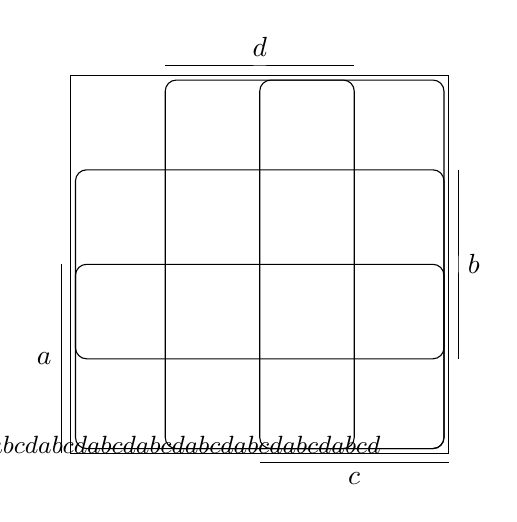
\begin{tikzpicture}[scale=1.2,every node/.style={rounded corners,fill=white}]
\begin{scope}[xshift=5cm]
  \draw(0,0)rectangle(4,4);%\draw[step=1mm, red] (0,0) grid (4,4);
  \draw[rounded corners,](0.05,0.05)rectangle(3.95,2);
  \draw(-0.1,0)--(-0.1,1)node[left]{$a$}--(-0.1,2);
 \draw(4.1,1)--(4.1,2)node[right]{$b$}--(4.1,3);
 \draw(2,-0.1)--(3,-0.1)node[below]{$c$}--(4,-0.1);
 \draw(1,4.1)--(2,4.1)node[above]{$d$}--(3,4.1);
  \draw[rounded corners,](2,0.05)rectangle(3.95,3.95); 
  \draw[rounded corners,](0.05,1)rectangle(3.95,3);
  \draw[rounded corners,](1,0.05)rectangle(3,3.95); 
\kmin{\small{$\comp{a}\comp{b}\comp{c}\comp{d}$}}{\small{$\comp{a}\comp{b}\comp{c}{d}$}}{\small{$\comp{a}\comp{b}{c}\comp{d}$}}{\small{$\comp{a}\comp{b}{c}{d}$}}{\small{$\comp{a}{b}\comp{c}\comp{d}$}}{\small{$\comp{a}{b}\comp{c}{d}$}}{\small{$\comp{a}{b}{c}\comp{d}$}}{\small{$\comp{a}{b}{c}{d}$}} %Coloca os valores dos quadros menos significativos
\kmax{\small{${a}\comp{b}\comp{c}\comp{d}$}}{\small{${a}\comp{b}\comp{c}{d}$}}{\small{${a}\comp{b}{c}\comp{d}$}}{\small{${a}\comp{b}{c}{d}$}}{\small{${a}{b}\comp{c}\comp{d}$}}{\small{${a}{b}\comp{c}{d}$}}{\small{${a}{b}{c}\comp{d}$}}{\small{${a}{b}{c}{d}$}} %Coloca os valores dos quadros mais significativos
 \end{scope}
\end{tikzpicture}
\caption{Diagrama Venn de 4 variáveis desenhado com regiões quadradas.}
	\label{fig:Venn4}
\end{figure}

O mapa de Karnaugh já é este diagrama de Venn modificado, onde o resultado da função booleana mapeada é marcado em cada região (casa). Cada casa em um mapa de Karnaugh corresponde a uma linha na tabela verdade, que é um AND de todas as variáveis envolvidas -- vamos chamar isto de mintermo. A figura \ref{fig:karnaugh_mintermos} mostra os mintermos correspondentes a cada uma das regiões.

\begin{figure}[hbt]
	\centering
  \begin{tikzpicture}[scale=1.2]
   \karnaugh{$a$}{$b$}{$c$}{$d$} %Faz um mapa de Karnaugh de 0 a 4
   \kmin{$\comp{a}\comp{b}\comp{c}\comp{d}$}{$\comp{a}\comp{b}\comp{c}{d}$}{$\comp{a}\comp{b}{c}\comp{d}$}{$\comp{a}\comp{b}{c}{d}$}{$\comp{a}{b}\comp{c}\comp{d}$}{$\comp{a}{b}\comp{c}{d}$}{$\comp{a}{b}{c}\comp{d}$}{$\comp{a}{b}{c}{d}$} %Coloca os valores dos quadros menos significativos
   \kmax{${a}\comp{b}\comp{c}\comp{d}$}{${a}\comp{b}\comp{c}{d}$}{${a}\comp{b}{c}\comp{d}$}{${a}\comp{b}{c}{d}$}{${a}{b}\comp{c}\comp{d}$}{${a}{b}\comp{c}{d}$}{${a}{b}{c}\comp{d}$}{${a}{b}{c}{d}$} %Coloca os valores dos quadros mais significativos
	 \end{tikzpicture}
	\caption{Mapa de Karnaugh com os mintermos correspondentes a cada casa.}
	\label{fig:karnaugh_mintermos}
\end{figure}

Note na figura \ref{fig:karnaugh_mintermos} que os vizinhos de cada casa em um mapa de Karnaugh são tais que apenas muda uma variável de cada vez. Por exemplo, da casa 5 para a 1 (acima) só muda o $b$, da 5 para a 7 (direita) só muda o $c$, da 5 para a 4 (esquerda) só muda o $d$ e da 5 para a 13 (abaixo) só muda o $a$. 

Isto que foi mostrado para a casa 5 é válido para todas casas, inclusive para as bordas e quinas, pois podemos considerar que o mapa dá a volta em si mesmo. Deste modo considera-se a casa 6 como vizinha da 4 e só muda a variável $c$, a casa 10 vizinha da 2 e só muda a variável $a$ e assim por diante.

Desta característica do mapa de Karnaugh vem sua principal utilidade. Por exemplo, considere a função $f_2=\Sigma_m(3,7,12,13)$ -- o somatório dos mintermos das casas 3, 7, 12 e 13 -- e seu respectivo mapa de karnaugh na figura \ref{fig:k_f2}.

\begin{figure}[hbt]
	\centering
  \begin{tikzpicture}[scale=0.8]
    \node() at(0,4)[above left]{$f_2=\Sigma_m(3,7,12,13)$}; 
   \karnaugh{$a$}{$b$}{$c$}{$d$} %Faz um mapa de Karnaugh de 0 a 4
   \kmin{0}{0}{0}{1}{0}{0}{0}{1} %Coloca os valores dos quadros menos significativos
   \kmax{0}{0}{0}{0}{1}{1}{0}{0} %Coloca os valores dos quadros mais significativos
   \grupo{0}{1}{2}{2}\node(p1)at (0.1,1.5){};
   \node(e1) at (-2,2){$ab\comp{c}$} edge[->,thick](p1);
	 \grupo{2}{2}{3}{4}\node(p2)at (2.9,3){};
	 \node(e2) at (6,3.5){$\comp{a}cd$} edge[->, thick](p2);
	 \end{tikzpicture}
	\caption{Função $f_2$ e simplificação por agrupamento de casas vizinhas.}
	\label{fig:k_f2}
\end{figure}

Analisando a função $f_2$ por álgebra de Boole, vemos que podemos simplificá-la através da aplicação do teorema que diz que $a\comp{b}+ab=a$ e, observando no mapa de Karnaugh, os termos que são unidos e simplificados são justamente os vizinhos.
\begin{equation*}
\begin{matrix}
f_2=&\!\!\!\underbrace{\comp{a}\comp{b}cd+\comp{a}bcd}&\!\!\!\!+&\!\!\!\!\underbrace{ab\comp{c}\comp{d}+ab\comp{c}d}\\
f_2=&\!\!\comp{a}cd&\!\!\!\!+&ab\comp{c}
\end{matrix}
\end{equation*}

Ou seja, o agrupamento de 2 casas vizinhas corresponde à simplificação de uma variável. Basta ver no próprio mapa quais são as variáveis que não mudam dentro do agrupamento.

Para simplificar 2 ou mais variáveis basta aplicar o teorema repetidas vezes. Simplifiquemos a função $f_3$ (vide figura \ref{fig:k_g_simples}), por exemplo. Basta agruparmos a função de duas em duas casas e 2 grupos vizinhos de duas casas viram um único grupo de 4 casas, retirando mais uma variável da função.

\begin{figure}[hbt]
\begin{align*}
f_3&=\underbrace{a\comp{b}\comp{c}\comp{d}+a\comp{b}\comp{c}{d}}+\underbrace{a{b}\comp{c}\comp{d}+a{b}\comp{c}{d}}\\
 &=\underbrace{a\comp{b}\comp{c}+a{b}\comp{c}}\\
 f_3&=a\comp{c}
\end{align*}
	\centering
	
\begin{center}
%	\begin{tabular}[c]{cc}
  \begin{tikzpicture}[scale=0.8]
    \node() at (0,4)[above left]{$f_3$};
   \karnaugh{$a$}{$b$}{$c$}{$d$} %Faz um mapa de Karnaugh de 0 a 4
   \kmin{0}{0}{0}{0}{0}{0}{0}{0} %Coloca os valores dos quadros menos significativos
   \kmax{1}{1}{0}{0}{1}{1}{0}{0} %Coloca os valores dos quadros mais significativos
   \grupo{0}{0}{2}{1}\node(p1)at (0.1,1.5){};
   \grupo{0}{1}{2}{2}\node(p1)at (0.1,1.5){};
%   \end{tikzpicture} %& 
%		  \begin{tikzpicture}[scale=0.8]
   \node(seta) at (6,2){\Huge $\Rightarrow$};
		\begin{scope}[xshift=8cm]
    \node() at (0,4)[above left]{$f_3$};
   \karnaugh{$a$}{$b$}{$c$}{$d$} %Faz um mapa de Karnaugh de 0 a 4
   \kmin{0}{0}{0}{0}{0}{0}{0}{0} %Coloca os valores dos quadros menos significativos
   \kmax{1}{1}{0}{0}{1}{1}{0}{0} %Coloca os valores dos quadros mais significativos
   \grupo{0}{0}{2}{2}\node(p1)at (0.1,1.5){};
   \end{scope}
   \end{tikzpicture}
%	\end{tabular}
\end{center}
	\caption{Agrupamento das casas da função $f_3$.}
	\label{fig:k_g_simples}
\end{figure}

Este mesmo procedimento pode ser mostrado para agrupamentos de 8 casas (simplificando então 3 variáveis) ou 16 casas (simplificando 4 variáveis.
A figura \ref{fig:k_exemplos}\footnote{Exemplos retirados do artigo original de Karnaugh: ``\emph{The map method for synthesis of combinational logic circuits}'', de 1953.} mostra algumas possibilidades de agrupamentos de 2, 4 e 8 casas, junto com o produto respectivo. Num mapa de Karnaugh de 4 variáveis um agrupamento de 16 casas seria todo o mapa e corresponderia a função 1.

\begin{figure}[hbtp]\begin{center}% 
\subfigure[agrupamentos de 2 casas]{
 \begin{tikzpicture}[scale=0.4]
   \draw(-0.1,4.1)node[above left]{$b\comp{c}d$};
   \karnaugh[0]{$a$}{$b$}{$c$}{$d$} %Faz um mapa de Karnaugh de 0 a 4
   \kmin{0}{0}{0}{0}{0}{1}{0}{0} %Coloca os valores dos quadros menos significativos
   \kmax{0}{0}{0}{0}{0}{1}{0}{0} %Coloca os valores dos quadros mais significativos
   \grupo[indefinido, rounded corners=1.5mm]{1}{1}{2}{3};
%   \quinas[indefinido, rounded corners=1.5mm]\node(p2)at (0.1,1.5){};
%   \end{tikzpicture} 

\begin{scope}[xshift=6cm]
   \draw(-0.1,4.1)node[above left]{$\comp{a}\comp{b}d$};
   \karnaugh[0]{$a$}{$b$}{$c$}{$d$} %Faz um mapa de Karnaugh de 0 a 4
   \kmin{0}{1}{0}{1}{0}{0}{0}{0} %Coloca os valores dos quadros menos significativos
   \kmax{0}{0}{0}{0}{0}{0}{0}{0} %Coloca os valores dos quadros mais significativos
   \grupo[indefinido, rounded corners=1.5mm]{1}{3}{3}{4}\node(p1)at (0.1,1.5){};
%   \grupo[indefinido, rounded corners=1.5mm]{1}{0}{2}{4}\node(p2)at (0.1,1.5){};
   \end{scope} 
\begin{scope}[xshift=12cm]
   \draw(-0.1,4.1)node[above left]{$\comp{a}\comp{b}\comp{d}$};
   \karnaugh[0]{$a$}{$b$}{$c$}{$d$} %Faz um mapa de Karnaugh de 0 a 4
   \kmin{1}{0}{1}{0}{0}{0}{0}{0} %Coloca os valores dos quadros menos significativos
   \kmax{0}{0}{0}{0}{0}{0}{0}{0} %Coloca os valores dos quadros mais significativos
   \lados[indefinido, rounded corners=1.5mm]{3}{4};

   \end{scope} 
\begin{scope}[xshift=18cm]
   \draw(-0.1,4.1)node[above left]{$\comp{b}\comp{c}\comp{d}$};
   \karnaugh[0]{$a$}{$b$}{$c$}{$d$} %Faz um mapa de Karnaugh de 0 a 4
   \kmin{1}{0}{0}{0}{0}{0}{0}{0} %Coloca os valores dos quadros menos significativos
   \kmax{1}{0}{0}{0}{0}{0}{0}{0} %Coloca os valores dos quadros mais significativos
   \topos[indefinido, rounded corners=1.5mm]{0}{1}\node(p1)at (0.1,1.5){};
%   \grupo[indefinido, rounded corners=1.5mm]{1}{0}{2}{4}\node(p2)at (0.1,1.5){};
   \end{scope}
\end{tikzpicture}}
\subfigure[Agrupamentos de 4 casas]{
 \begin{tikzpicture}[scale=0.4] 
 \begin{scope}
   \draw(-0.1,4.1)node[above left]{$\comp{c}d$};
   \karnaugh[0]{$a$}{$b$}{$c$}{$d$} %Faz um mapa de Karnaugh de 0 a 4
   \kmin{0}{1}{0}{0}{0}{1}{0}{0} %Coloca os valores dos quadros menos significativos
   \kmax{0}{1}{0}{0}{0}{1}{0}{0} %Coloca os valores dos quadros mais significativos
   \grupo[indefinido, rounded corners=1.5mm]{1}{0}{2}{4};
  
 \begin{scope}[xshift=6cm]
   \draw(-0.1,4.1)node[above left]{$a\comp{b}$};
   \karnaugh[0]{$a$}{$b$}{$c$}{$d$} %Faz um mapa de Karnaugh de 0 a 4
   \kmin{0}{0}{0}{0}{0}{0}{0}{0} %Coloca os valores dos quadros menos significativos
   \kmax{1}{1}{1}{1}{0}{0}{0}{0} %Coloca os valores dos quadros mais significativos
   \grupo[indefinido, rounded corners=1.5mm]{0}{0}{4}{1};
     \end{scope}
 \begin{scope}[xshift=12cm]
   \draw(-0.1,4.1)node[above left]{$\comp{a}\,\comp{d}$};
   \karnaugh[0]{$a$}{$b$}{$c$}{$d$} %Faz um mapa de Karnaugh de 0 a 4
   \kmin{1}{0}{1}{0}{1}{0}{1}{0} %Coloca os valores dos quadros menos significativos
   \kmax{0}{0}{0}{0}{0}{0}{0}{0} %Coloca os valores dos quadros mais significativos
   \lados[indefinido, rounded corners=1.5mm]{2}{4};
     \end{scope}
 \begin{scope}[xshift=18cm]
   \draw(-0.1,4.1)node[above left]{$\comp{b}\,\comp{d}$};
   \karnaugh[0]{$a$}{$b$}{$c$}{$d$} %Faz um mapa de Karnaugh de 0 a 4
   \kmin{1}{0}{1}{0}{0}{0}{0}{0} %Coloca os valores dos quadros menos significativos
   \kmax{1}{0}{1}{0}{0}{0}{0}{0} %Coloca os valores dos quadros mais significativos
   \quinas[indefinido, rounded corners=1.5mm];
     \end{scope}
   \end{scope} 
\end{tikzpicture}}
\subfigure[Agrupamentos de 8 casas]{
 \begin{tikzpicture}[scale=0.4] 
 \begin{scope}
   \draw(-0.1,4.1)node[above left]{$b$};
   \karnaugh[0]{$a$}{$b$}{$c$}{$d$} %Faz um mapa de Karnaugh de 0 a 4
   \kmin{0}{0}{0}{0}{1}{1}{1}{1} %Coloca os valores dos quadros menos significativos
   \kmax{0}{0}{0}{0}{1}{1}{1}{1} %Coloca os valores dos quadros mais significativos
   \grupo[indefinido, rounded corners=1.5mm]{0}{1}{4}{3};
  
 \begin{scope}[xshift=6cm]
   \draw(-0.1,4.1)node[above left]{$\comp{d}$};
   \karnaugh[0]{$a$}{$b$}{$c$}{$d$} %Faz um mapa de Karnaugh de 0 a 4
   \kmin{1}{0}{1}{0}{1}{0}{1}{0} %Coloca os valores dos quadros menos significativos
   \kmax{1}{0}{1}{0}{1}{0}{1}{0} %Coloca os valores dos quadros mais significativos
   \lados[indefinido, rounded corners=1.5mm]{0}{4};
     \end{scope}
 \begin{scope}[xshift=12cm]
   \draw(-0.1,4.1)node[above left]{$c$};
   \karnaugh[0]{$a$}{$b$}{$c$}{$d$} %Faz um mapa de Karnaugh de 0 a 4
   \kmin{0}{0}{1}{1}{0}{0}{1}{1} %Coloca os valores dos quadros menos significativos
   \kmax{0}{0}{1}{1}{0}{0}{1}{1} %Coloca os valores dos quadros mais significativos
   \grupo[indefinido, rounded corners=1.5mm]{2}{0}{4}{4};
     \end{scope}
 \begin{scope}[xshift=18cm]
   \draw(-0.1,4.1)node[above left]{$\comp{b}$};
   \karnaugh[0]{$a$}{$b$}{$c$}{$d$} %Faz um mapa de Karnaugh de 0 a 4
   \kmin{1}{1}{1}{1}{0}{0}{0}{0} %Coloca os valores dos quadros menos significativos
   \kmax{1}{1}{1}{1}{0}{0}{0}{0} %Coloca os valores dos quadros mais significativos
   \topos[indefinido, rounded corners=1.5mm]{0}{4};
     \end{scope}
   \end{scope} 
   \end{tikzpicture}}
\caption{Exemplos de mapas de karnaugh com os correspondentes produtos algébricos.}\label{fig:k_exemplos}
\end{center}
\end{figure}
\clearpage

\subsection{Mapas de $n$ variáveis}

É fácil fazer um mapa de Karnaugh com um número menor de variáveis (i.e.: $n<4$). Para tanto basta simplesmente sair dividindo o mapa. Deve-se apenas lembrar que uma casa deve ter $n$ vizinhas, já que a simplificação de uma variável corresponde a unir uma casa com a vizinha. Isto é mostrado na figura \ref{fig:karnaughzinhos} para mapas de 2, 3 e 4 variáveis.

\begin{figure}[!h]
\centering
\subfigure[Mapa de 2 variáveis]{
 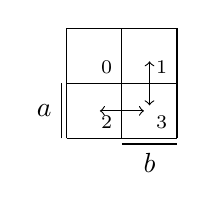
\begin{tikzpicture}[scale=0.7] 
\draw[step=1cm, black] (0,0) grid (2,2); %defining grids
  \draw(-0.1,0)--(-0.1,0.5)node[left]{$a$}--(-0.1,1);
  \draw(1,-0.1)--(1.5,-0.1)node[below]{$b$}--(2,-0.1);

  \draw(1,1)node[above left]{\scriptsize 0};
  \draw(2,1)node[above left]{\scriptsize 1};
  \draw(1,0)node[above left]{\scriptsize 2};
  \draw(2,0)node[above left]{\scriptsize 3};
  \draw[<->](1.5,0.6)--(1.5,1.4);
  \draw[<->](0.6,0.5)--(1.4,0.5);
 \end{tikzpicture}}
\subfigure[Mapa de 3 variáveis]{
 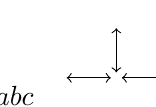
\begin{tikzpicture}[scale=0.7] 
   \karnaughtres{$a$}{$b$}{$c$}
   \draw[<->](1.5,0.6)--(1.5,1.4);
   \draw[<->](0.6,0.5)--(1.4,0.5);
   \draw[<->](1.6,0.5)--(2.4,0.5);
 \end{tikzpicture}}
\subfigure[Mapa de 4 variáveis]{
 \begin{tikzpicture}[scale=0.7] 
   \karnaugh[1]{$a$}{$b$}{$c$}{$d$} %Faz um mapa de Karnaugh de 0 a 4
   \draw[<->](1.5,2.6)--(1.5,3.4);
   \draw[<->](1.5,1.6)--(1.5,2.4);
   \draw[<->](0.6,2.5)--(1.4,2.5);
   \draw[<->](1.6,2.5)--(2.4,2.5);
 \end{tikzpicture}}
\caption{Mapas de Karnaugh de $n= 2, 3, 4$ variáveis, mostrando que cada casa tem $n$ vizinhas.}
\label{fig:karnaughzinhos}
\end{figure}

Mas como aplicar este princípio para funções com mais de 4 variáveis? É impossível fazer um mapa no plano onde cada uma das regiões tem 5 (ou mais) vizinhos. Uma maneira (não muito prática) é trabalhar com um mapa tridimensional como exemplifica a figura \ref{fig:karnaugh6_3d} que mostra um mapa de Karnaugh de 6 variáveis, note que cada casa tem 6 vizinhos: 4 no plano (como no mapa de 4 variáveis) e 2 verticais.

\begin{figure}
\centering

 \begin{tikzpicture}
  \begin{scope}[yscale=0.4,xshift=0cm,xslant=0.5]
   \karnaugh[3]{$c$}{$d$}{$e$}{$f$}
  \end{scope}
  \begin{scope}[yshift=2.25cm,yscale=0.4,xshift=0cm,xslant=0.5]
   \karnaugh[4]{$c$}{$d$}{$e$}{$f$}
  \end{scope}
  \begin{scope}[yshift=4.5cm,yscale=0.4,xshift=0cm,xslant=0.5]
   \karnaugh[2]{$c$}{$d$}{$e$}{$f$}
  \end{scope}
  \begin{scope}[yshift=6.75cm,yscale=0.4,xshift=0cm,xslant=0.5]
   \karnaugh[1]{$c$}{$d$}{$e$}{$f$}
  \end{scope}
\draw(-0.25,-0.25)--(-0.25,2)node[left]{$a$}--(-0.25,4.25);
\draw(6.25,2)--(6.25,4.25)node[right]{$b$}--(6.25,6.5);
%\draw[color=white](-1,0)--(-1.5,1);

 \end{tikzpicture}
\caption{Mapa de Karnaugh tridimensional de 6 variáveis.}\label{fig:karnaugh6_3d}
\end{figure}


Na prática, um mapa de 5 variáveis é desenhado como 2 de 4 variáveis, sendo um com uma variável (em geral a mais significativa) sendo 0 e o outro com a mesma variável sendo 1. Usa-se este mesmo princípio para mapas de 6 ou mais variáveis, como pode ser visto na figura \ref{fig:karnaughzaos}.

\begin{figure}
\centering
\subfigure[5 variáveis]{
 \begin{tikzpicture}[scale=0.45]
  \begin{scope}[xshift=0cm]
   \karnaugh[1]{$b$}{$c$}{$d$}{$e$}
  \end{scope}
  \begin{scope}[yshift=0cm,xshift=6cm]
   \karnaugh[2]{$b$}{$c$}{$d$}{$e$}
  \end{scope}
\draw(5.5,5.5)--(8,5.5)node[above]{$a$}--(10.5,5.5);
\end{tikzpicture}
}
\subfigure[6 variáveis]{
 \begin{tikzpicture}[scale=0.45]
  \begin{scope}[xshift=0cm]
   \karnaugh[3]{$c$}{$d$}{$e$}{$f$}
  \end{scope}
  \begin{scope}[yshift=0cm,xshift=6cm]
   \karnaugh[4]{$c$}{$d$}{$e$}{$f$}
  \end{scope}
  \begin{scope}[yshift=6cm,xshift=6cm]
   \karnaugh[2]{$c$}{$d$}{$e$}{$f$}
  \end{scope}
  \begin{scope}[yshift=6cm,xshift=0cm]
   \karnaugh[1]{$c$}{$d$}{$e$}{$f$}
  \end{scope}
\draw(-1.5,-0.5)--(-1.5,2)node[left]{$a$}--(-1.5,4.5);
\draw(5.5,11.5)--(8,11.5)node[above]{$b$}--(10.5,11.5);


 \end{tikzpicture}}
\caption{Mapas de Karnaugh de 5 e 6 variáveis.}\label{fig:karnaughzaos}
\end{figure}
\clearpage

\section{Equações e circuitos não-completamente especificados.}
\label{sec:nao-completamente}

É bastante comum a situação de que determinadas entradas de um circuito lógico nunca ocorram. Como exemplo imagine-se uma esteira carregando uma caixa de um lado para o outro, com sensores de fim de curso em ambas extremidades: $s_e$ do lado esquerdo e $s_d$ do lado direito. No funcionamento normal do sistema estes dois sinais nunca serão acionados ao mesmo tempo; nesta situação não importa qual é o resultado do circuito para $s_e=s_d=1$, já que esta situação nunca vai existir. Diz-se então que este circuito é não-completamente especificado.

A tabela \ref{tab:verdade_nce} mostra o exemplo de um sinal imaginário $z$ determinado em função de $a$, $s_e$ e $s_d$. Neste exemplo, sempre que $s_e=s_d=1$ a saída $z$ é não-especificada, ou seja, $z$ \emph{não-importa} nestas situações. Neste texto utilizaremos a notação `$\times$' para identificar as situações que um sinal não importa. Outras notações comumente usadas são `$\ast$', `-' ou `$d$'.

\begin{table}[!h]
  \centering
  \caption{Exemplo de uma função não completamente especificada.}
  \label{tab:verdade_nce}
    \begin{tabular}{|c|c|c||c|}
\hline
$a$ & $s_e$ & $s_d$ & $z$ \\
\hline\hline
0 & 0 & 0 & 0 \\

0 & 0 & 1 & 0 \\

0 & 1 & 0 & 1 \\

0 & 1 & 1 & $\times$ \\
\hline
1 & 0 & 0 & 1 \\

1 & 0 & 1 & 0 \\

1 & 1 & 0 & 1 \\

1 & 1 & 1 & $\times$ \\
\hline
\end{tabular}
\end{table}

Pode-se descrever uma função lógica não-completamente especificada na forma soma de mintermos utilizando a notação $d(\cdots)$, que vem do inglês \emph{don't care}. Desta forma o sinal z pode ser descrito por:
\begin{equation}
  \label{eq:z}
  z = \Sigma_m(2,4,6)+d(3,7)
\end{equation}

Um \dontcare~na saída pode ser implementado como um 1 ou um 0, e não se sabe a princípio qual destes dois valores gerará uma solução mais minimizada, logo para obter o menor circuito possível o engenheiro deveria, a princípio, obter as equações considerando que cada \dontcare~pode ser 1 ou 0 e checar qual é o menor circuito final. Obviamente para problemas com muitos \dontcare's isto se torna impraticável, pois seria necessário minimizar $2^k$ funções, onde $k$ é o número de \dontcare's presentes.

O mapa de Karnaugh facilita bastante a implementação de circuitos não-completamente especificados, pois podemos considerar se determinado \dontcare~é 1 ou 0 visualmente, na hora da implementação.


\begin{figure}[!h]
  \centering
  \begin{tikzpicture}
    \node() at (0,2)[above left]{$z$};
    \karnaughtres{$a$}{$s_e$}{$s_d$}
    \kmax{1}{0}{1}{$\times$}{0}{0}{1}{$\times$}

%    \grupo[zeros]{1}{0}{3}{2}
%    \grupo[zeros]{0}{1}{2}{2}

    \grupo{2}{0}{4}{2}
    \lados{0}{1}

  \end{tikzpicture}
  \caption{Mapa de Karnaugh da função $z$.}
  \label{fig:kmap_z}
\end{figure}

\section{Linguagem Ladder – Temporizadores}
\section{Linguagem Ladder – Contadores}
\section{Linguagem Ladder – Aplicações}
%!TEX root = principal.tex
\chapter{Linguagem grafcet}

GRAphe Fonctionnel de Commande Etape/Transition - Grafo funcional de comando etapa/transição, é um formalismo matemático tal como uma máquina de etapas. Tem origem na chamada máquina de etapas, mas com mais funcionalidades, tais como a possibilidade de ter etapas em paralelo e de ter macro-etapas.

Um diagrama grafcet é composto dos seguintes elementos: etapas, transições, ações, divergências e convergências E e divergências e convergências OU.

O básico do grafcet é a sequência etapa-transição-etapa, como mostra na figura \ref{fig:grafcetSimples}. Ela apresenta um diagrama grafcet com 3 etapas (os quadrados) e três transições (os retângulos verde e vermelhos). Etapas e transições podem estar ativas ou não. Etapas ativas são representadas com uma ficha dentro delas (vide Etapa 1 na figura), enquanto que transições ativas são em geral representadas por uma mudança de cor. Neste exemplo uma transição ativa é representada pela cor verde, enquanto uma inativa é representada pela cor vermelha.

A ativação de uma transição é diretemente relacionada a uma condição lógica associada a mesma: quando veradeiras, as ativam. Já a ativação das etapas depende da dinâmica do sistema. No exemplo da figura \ref{fig:grafcetSimples}, A Etapa 0 é uma etapa inicial (representado pela linha dupla), significando que o sistema inicia com a Etapa 0 ativa, mas não as demais. No momento mostrado na figura \ref{fig:grafcetSimples}, a Etapa 1 é que está ativa, indicado pela ficha.

\begin{figure}[hbt]
  \centering
  \includegraphics[scale=0.6]{figuras/grafcetSimples}
  \caption{Exemplo de um diagrama grafcet simples.}
  \label{fig:grafcetSimples}
\end{figure}

A evolução do sistema descrito em grafcet é dada pelo disparo das transições. Um transição dispara quando:
\begin{itemize}
  \item ela está ativa (ou seja, a condição ligada a ela é verdadeira) e
  \item todos as etapas anteriores a ela estão ativas.
\end{itemize}

Quando uma transição dispara ela desativa todos os etapas anteriores a ela (as etapas acima) e ativa todos as posteriores (as abaixo). Por exemplo, se na figura \ref{fig:grafcetSimples} a condição A se tornasse verdadeira, como a única etapa anterior (a Etapa 1) está ativa, esta transição dispararia, desativando a Etapa 1 e ativando a Etapa 2. Esta sequência é mostrada na figura \ref{fig:grafcetDisparo}.
\begin{figure}[hbt]
  \centering
  \includegraphics[scale=0.6]{figuras/grafcetDisparo}
  \caption{Sequência de disparo da transição A}
  \label{fig:grafcetDisparo}
\end{figure}

\section{Divergências e convergências}

No grafcet, pode-se ter uma etapa com mais de uma transição de saída, que pode levar para etapas diferentes de acordo com qual transição dispare primeiro. A isto se chama uma \emph{divergência OU}, pois separa em dois caminhos excludentes. Da mesma forma, duas (ou mais) transições podem levar para o mesmo etapa, o que se chama de convergência OU. A figura \ref{fig:grafcetdivOU} mostra um exemplo em que o sistema pode evoluir por dois caminhos diferentes, com o uso de divergência e convergência OU.

\begin{figure}[hbt]
  \centering
  \includegraphics[scale=0.6]{figuras/grafcetdivOU}
  \caption{Exemplo de grafcet com divergência e convergência OU. O !A indica que a transição está ativa quando A for falso.}
  \label{fig:grafcetdivOU}
\end{figure}

Note-se na figura \ref{fig:grafcetdivOU} que a Etapa 1 é obrigatoriamente transitória, pois ou A é verdadeiro e o sistema evolui imediatamente para o etapa 2 ou A é falso e o sistema ativa o etapa 3. É possível definir transições que estejam ativas ao mesmo tempo, neste caso o sistema evolui para a transição com maior prioridade -- ou a mais a esquerda ou se tiver uma prioridade explícita.

Diferente de uma máquina de estados, no grafcet é permitido que uma transição acione mais que uma etapa. Neste caso o sistema se divide em caminhos paralelos. Isto é chamado de divergência E e indicado por duas linhas horizontais, para diferenciar da divergência OU. Da mesma forma, uma convergência E liga várias etapas a uma única transição, transformando caminhos paralelos num único caminho. A figura \ref{fig:grafcetdivE} mostra um exemplo de divergência e convergência E.

\begin{figure}[hbt]
  \centering
  \includegraphics[scale=0.6]{figuras/grafcetdivE}
  \caption{Exemplo de grafcet com divergência e convergência E.}
  \label{fig:grafcetdivE}
\end{figure}

Neste caso, mesmo com P ativo, o sistema não desativa a Etapa 2a nem ativa a Etapa 0, pois como a Etapa 2b não está ativa, a transição P não pode disparar.

\section{Ações}
Outra característica do grafcet é que podem ser definidas ações, ligadas a etapas. O que exatamente compõem uma ação depende da implementação do grafcet. Peguemos dois exemplos: o JGrafchart e a SFC, que é a descrição de grafcet definida pela norma IEC61131.

\subsection{JGrafchart}
\label{sub:JGrafchart}

No JGrafchart, uma ação pode ser uma definição de valor (um \emph{assignment}), da forma \lstinline|variavel = expressao|, uma chamada de subrotina (\emph{call}) ou uma variável booleana (\emph{bool}), que fica verdadeira enquanto a etapa estiver ativa. Um qualificador de uma letra define o momento em que a ação é executada:
\begin{description}
  \item[S assignment|call;] Executa apenas uma vez, quando a etapa é ativada.
  \item[X assignment|call;] Executa apenas uma vez, quando a etapa é desativada.
  \item[P assignment|call;] Executa a cada ciclo enquanto a ação estiver acionada.
  \item[N bool;] Torna verdadeira a variável booleana enquanto a etapa estiver acionada.
  \item[A assignment|call;] Executa apenas uma vez, se a etapa for desativada por uma transição de exceção (apenas definida no JGrafchart).
\end{description}

Note-se que a ação \lstinline/N bool;/ é equivalente a \lstinline/S bool=1; X bool=0;/ e é presente para facilitar a escrita, já que tal operação é feita muitas vezes.

Toda etapa tem uma variável booleana x (\lstinline|<nome_da_etapa>.x|), que é verdadeira quando a etapa é acionada, e uma variável de tempo em décimos de segundo t (\lstinline|<nome_da_etapa>.t|) e em segundos s (\lstinline|<nome_da_etapa>.s|) que contam o tempo desde que a etapa iniciou.

\subsection{SFC}
\label{sub:SFC}

As ações do SFC são do formato \textbf{\lstinline/qualificador funcao|variavel finalizado/}. \lstinline|finalizado| é uma variável opcional no caso de se usar uma função, que aciona quando a função termina, o que a torna útil para ser utilizada na transição de saída da etapa.

O qualificador pode ser qualquer um dos descritos na tabela \ref{tab:qualiSFC}. Pode-se não especificar o qualificador, onde o comportamento fica o mesmo de se usar o qualificador N. No caso da ação ser uma função, ele é executada sempre que ficar ativa. Todos os qualificadores que tem tempo acompanham um valor de tempo dado ou por uma variável ou por uma constante da forma \lstinline|T#4k|, onde k pode ser t (décimo de segundo), s (segundo), m, (minuto) ou h (hora).
\begin{table}[hbt]
  \caption{Qualificadores do SFC}
  \label{tab:qualiSFC}
  \centering

  \begin{tabularx}{\textwidth}{|c|X|}
  \hline

  \hline
  \textbf{Qualificador} & \textbf{descrição}\\
  \hline
   \textbf{N}  & Ativa a etapa estiver acionada. \\
   \textbf{S}  & Set -- ativa e mantém ativado mesmo depois de sair da etapa. \\
   \textbf{R}  & Reset -- desativa. \\
   \textbf{P}  & Ativa apenas no primeiro ciclo que a etapa estiver ativa. \\
   \textbf{L tempo}  & Ativa pelo tempo determinado enquanto a etapa estiver acionada.\\
   \textbf{SL tempo}  & Ativa pelo tempo determinado independente da etapa ainda estar acionada.\\
   \textbf{D tempo}  & Ativa após o tempo determinado enquanto a etapa estiver acionada.\\
   \textbf{SD tempo}  & Seta após o tempo determinado independente da etapa ainda estar acionada.\\
   \textbf{DS tempo}  & Seta após o tempo determinado se a etapa ainda estiver acionada.\\
  \hline

  \hline
  \end{tabularx}
\end{table}

\clearpage
\section{Níveis}
O Grafcet pode ser definido em 2 níveis de abstração: o 1 e o 2. O nível 1 serve como uma ferramenta de desenvolvimento, para analisar a partir do problema como um todo a sequência de etapas, as ações a serem realizadas em cada etapa e as condições de transição de uma etapa para outra. No nível 1 as ações e transições são descritas de forma ampla, para permitirem uma melhor visualização do processo pelo desenvolvedor. O resultado final é uma descrição dos requisitos daquelas etapas e transições e não serve como uma linguagem para programar um sistema.

Já o Grafcet nível 2 é propriamente uma linguagem de programação, com diferentes implementações. Uma delas é o SFC - \emph{Sequential Function Chart}, descrita no padrão IEC1131-3 para programação de CLPs. No SFC, cada ação corresponde a uma atuação nas saídas ou variáveis internas do CLP e cada transição corresponde a um valor binário obtido no CLP seja de entradas, seja de comparações de valores analógicos ou de tempo.

Desta forma o principal uso do grafcet é num projeto top-down, onde a partir do problema se desenvolve a sequência a ser seguida no grafcet nível 1, a partir deste se definem todas as entradas, saídas e condições necessárias para o controle automático daquela sequência e então programa-se o sistema usando grafcet nível 2.

Tomemos como exemplo uma tarefa relativamente simples: cozinhar um ovo. Considere-se o sistema da figura \ref{fig:cozinhar_ovo}, consistindo de uma panela, uma entrada de água, uma boca de fogão a gás e um mecanismo que solte o ovo na água.

\begin{figure}[!h]
\centering
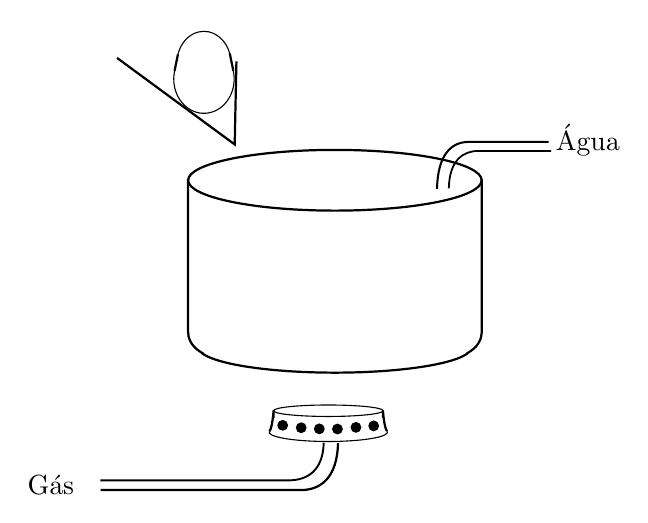
\begin{tikzpicture}[y=0.80pt, x=0.8pt,xscale=0.8,yscale=-0.8, inner sep=0pt, outer sep=0pt]
\begin{scope}[shift={(-99.03245,-288.02393)}]
    \path[draw=black,line join=miter,line cap=butt,line width=0.800pt]
      (354.2857,372.3622) .. controls (354.2857,381.8299) and (317.1893,389.5050) ..
      (271.4286,389.5050) .. controls (225.6678,389.5050) and (188.5714,381.8299) ..
      (188.5714,372.3622) .. controls (188.5714,362.8944) and (225.6678,355.2193) ..
      (271.4286,355.2193) .. controls (317.1893,355.2193) and (354.2857,362.8944) ..
      (354.2857,372.3622) -- cycle;
    \path[cm={{0.93174,0.0,0.0,0.83675,(18.52752,155.07504)}},draw=black,line
      join=miter,line cap=butt,line width=0.800pt] (351.5135,376.7594) .. controls
      (339.7757,385.9104) and (294.4050,391.3600) .. (250.1753,388.9315) .. controls
      (220.3437,387.2935) and (197.3850,382.3608) .. (190.5989,376.1313);
    \path[draw=black,line join=miter,line cap=butt,line width=0.800pt]
      (188.4845,371.6696) .. controls (188.4845,371.6696) and (188.4845,450.0421) ..
      (188.4845,457.6107) .. controls (188.4845,461.2730) and (190.0955,465.6973) ..
      (194.9956,468.8884) .. controls (198.4879,471.1627) and (197.0297,470.3066) ..
      (197.0297,470.3066);
    \path[draw=black,line join=miter,line cap=butt,line width=0.800pt]
      (354.3736,371.7266) .. controls (354.3736,371.7266) and (354.3736,450.0990) ..
      (354.3736,457.6677) .. controls (354.3736,461.3300) and (352.7625,465.7543) ..
      (347.8624,468.9454) .. controls (344.3701,471.2196) and (345.8283,470.3635) ..
      (345.8283,470.3635);
  \path[draw=black,line join=miter,line cap=butt,line width=0.800pt]
    (148.4437,303.3074) -- (214.8527,352.1376) -- (215.8294,305.2606);
  \begin{scope}[cm={{0.52126,0.0,0.0,0.55799,(132.31437,-4.68415)}}]
    \path[shift={(-3.38483,0)},draw=black] (160.1446,564.8529) .. controls
      (164.5668,583.4180) and (153.9497,602.2669) .. (136.4306,606.9532) .. controls
      (118.9114,611.6395) and (101.1244,600.3885) .. (96.7021,581.8235) .. controls
      (95.2554,575.7501) and (95.3885,569.3749) .. (97.0871,563.3753);
    \path[cm={{0.89621,0.0,0.0,-0.93321,(9.92999,1092.4228)}},draw=black]
      (160.3532,580.8939) .. controls (156.4154,599.5810) and (138.9277,611.3472) ..
      (121.2933,607.1743) .. controls (108.9462,604.2525) and (99.2953,594.0489) ..
      (96.5099,580.9713);
    \path[draw=black,line join=miter,line cap=butt,line width=0.800pt]
      (93.2329,565.0164) -- (96.8536,548.3611);
    \path[draw=black,line join=miter,line cap=butt,line width=0.800pt]
      (156.8450,565.0164) -- (153.0433,547.4560);
  \end{scope}
  \begin{scope}[shift={(0,10.0)}]
    \path[shift={(165.51847,-28.86265)},draw=black] (133.1216,521.3483) .. controls
      (133.1216,523.1376) and (119.2763,524.5880) .. (102.1973,524.5880) .. controls
      (85.1183,524.5880) and (71.2731,523.1376) .. (71.2731,521.3483) .. controls
      (71.2731,519.5591) and (85.1183,518.1086) .. (102.1973,518.1086) .. controls
      (119.2763,518.1086) and (133.1216,519.5591) .. (133.1216,521.3483) -- cycle;
    \path[cm={{0.95437,0.0,0.0,1.00307,(10.48141,-1.55578)}},draw=black]
      (304.2515,503.8934) .. controls (306.6885,506.7980) and (293.0976,509.4514) ..
      (273.8954,509.8200) .. controls (254.6932,510.1886) and (237.1512,508.1328) ..
      (234.7143,505.2283) .. controls (234.3214,504.7600) and (234.3437,504.2859) ..
      (234.7807,503.8186);
    \path[draw=black,line join=miter,line cap=butt,line width=0.800pt]
      (234.4953,503.9994) .. controls (236.1212,502.2258) and (236.7863,492.5444) ..
      (236.7863,492.5444) .. controls (236.7863,492.5444) and (236.7863,501.7823) ..
      (236.7863,492.2488);
    \path[draw=black,line join=miter,line cap=butt,line width=0.800pt]
      (300.8602,503.9994) .. controls (299.2343,502.2258) and (298.5692,492.5444) ..
      (298.5692,492.5444) .. controls (298.5692,492.5444) and (298.5692,501.7823) ..
      (298.5692,492.2488);
    \path[shift={(37.28111,-18.91723)},draw=black,fill=black] (248.7459,520.7984) ..
      controls (248.7459,522.2992) and (247.5293,523.5158) .. (246.0286,523.5158) ..
      controls (244.5278,523.5158) and (243.3112,522.2992) .. (243.3112,520.7984) ..
      controls (243.3112,519.2976) and (244.5278,518.0810) .. (246.0286,518.0810) ..
      controls (247.5293,518.0810) and (248.7459,519.2976) .. (248.7459,520.7984) --
      cycle;
    \path[shift={(26.8373,-17.9766)},draw=black,fill=black] (248.7459,520.7984) ..
      controls (248.7459,522.2992) and (247.5293,523.5158) .. (246.0286,523.5158) ..
      controls (244.5278,523.5158) and (243.3112,522.2992) .. (243.3112,520.7984) ..
      controls (243.3112,519.2976) and (244.5278,518.0810) .. (246.0286,518.0810) ..
      controls (247.5293,518.0810) and (248.7459,519.2976) .. (248.7459,520.7984) --
      cycle;
    \path[shift={(16.60251,-18.08111)},draw=black,fill=black] (248.7459,520.7984) ..
      controls (248.7459,522.2992) and (247.5293,523.5158) .. (246.0286,523.5158) ..
      controls (244.5278,523.5158) and (243.3112,522.2992) .. (243.3112,520.7984) ..
      controls (243.3112,519.2976) and (244.5278,518.0810) .. (246.0286,518.0810) ..
      controls (247.5293,518.0810) and (248.7459,519.2976) .. (248.7459,520.7984) --
      cycle;
    \path[shift={(6.36773,-18.7082)},draw=black,fill=black] (248.7459,520.7984) ..
      controls (248.7459,522.2992) and (247.5293,523.5158) .. (246.0286,523.5158) ..
      controls (244.5278,523.5158) and (243.3112,522.2992) .. (243.3112,520.7984) ..
      controls (243.3112,519.2976) and (244.5278,518.0810) .. (246.0286,518.0810) ..
      controls (247.5293,518.0810) and (248.7459,519.2976) .. (248.7459,520.7984) --
      cycle;
    \path[shift={(-4.07609,-20.0669)},draw=black,fill=black] (248.7459,520.7984) ..
      controls (248.7459,522.2992) and (247.5293,523.5158) .. (246.0286,523.5158) ..
      controls (244.5278,523.5158) and (243.3112,522.2992) .. (243.3112,520.7984) ..
      controls (243.3112,519.2976) and (244.5278,518.0810) .. (246.0286,518.0810) ..
      controls (247.5293,518.0810) and (248.7459,519.2976) .. (248.7459,520.7984) --
      cycle;
    \path[shift={(47.30687,-19.75335)},draw=black,fill=black] (248.7459,520.7984) ..
      controls (248.7459,522.2992) and (247.5293,523.5158) .. (246.0286,523.5158) ..
      controls (244.5278,523.5158) and (243.3112,522.2992) .. (243.3112,520.7984) ..
      controls (243.3112,519.2976) and (244.5278,518.0810) .. (246.0286,518.0810) ..
      controls (247.5293,518.0810) and (248.7459,519.2976) .. (248.7459,520.7984) --
      cycle;
  \end{scope}
  \path[draw=black,line join=miter,line cap=butt,line width=0.800pt]
    (273.1769,520.7233) .. controls (272.7485,540.4295) and (263.3238,547.2838) ..
    (252.1855,547.2838) .. controls (241.0472,547.2838) and (139.0890,547.2838) ..
    (139.0890,547.2838);
  \path[draw=black,line join=miter,line cap=butt,line width=0.692pt]
    (265.1049,520.6557) .. controls (264.7021,536.3302) and (255.8400,541.7823) ..
    (245.3666,541.7823) .. controls (234.8932,541.7823) and (139.0214,541.7823) ..
    (139.0214,541.7823);
  \path[fill=black] (97.967995,549.99866) node[above right] (text3077) {Gás};
  \path[draw=black,line join=miter,line cap=butt,line width=0.736pt]
    (329.0890,377.2838) .. controls (329.4517,357.5776) and (337.4309,350.7233) ..
    (346.8607,350.7233) .. controls (356.2906,350.7233) and (392.0864,350.7233) ..
    (392.0864,350.7233);
  \path[draw=black,line join=miter,line cap=butt,line width=0.638pt]
    (335.7362,376.9255) .. controls (336.0789,361.2509) and (343.6164,355.7989) ..
    (352.5243,355.7989) .. controls (361.4323,355.7989) and (393.4609,355.7989) ..
    (393.4609,355.7989);
  \path[fill=black] (396.19095,358.56888) node[above right] (text3085) {Água};
\end{scope}

\end{tikzpicture}
\caption{Sistema para cozinhar ovo sem sensores ou atuadores.}
\label{fig:cozinhar_ovo}
\end{figure}

Podemos inicialmente fazer um grafcet considerando que tudo dá sempre certo: ao iniciarmos o sistema, a panela enche de água, o ovo é colocado, o fogo acendido e aguarda-se até o ovo ficar pronto, de onde se retira a panela para tirar o ovo. Esta sequência é descrita pelo grafcet da figura \ref{fig:grafcetOvoOK}.

\begin{figure}[!h]
\centering
\includegraphics[scale=1]{figuras/ovoOK}
\caption{Diagrama grafcet nível 1 para cozinhar um ovo de forma otimista.}
\label{fig:grafcetOvoOK}
\end{figure}

Porém, problemas acontecem. Pode-se, por exemplo, esquecer de colocar a panela de volta antes de iniciar, faltar fogo ou acabar o ovo. Colocando todas estas condições a mais e defininindo o que fazer se elas acontecerem o grafcet cresce para o apresentado na figura \ref{fig:grafcetOvo1}.

\begin{figure}[!h]
\centering
\includegraphics[scale=1]{figuras/ovoNivel1}

\caption{Diagrama grafcet nível 1 para cozinhar um ovo.}
\label{fig:grafcetOvo1}
\end{figure}

Com base neste diagrama, pode-se analisar agora quais são os sensores e atuadores necessários para esta tarefa, mostrados na figura \ref{fig:cozinhar_ovo2}. São eles:

\begin{description}
  \item[S\_PP] Sensor de presença para detectar a panela.
  \item[S\_N] Sensor de distância para obter o nível de água.
  \item[S\_G] Sensor de gás.
  \item[B\_I] Botão de início.
  \item[B\_OK] Botão de OK, para continuar se der bronca.
  \item[B\_C] Botão de cancelamento.
  \item[PO] Solenóide para abrir a portinhola do ovo.
  \item[VA] Válvula de controle da água.
  \item[VG] Válvula de controle do gás.
  \item[CENTELHA] para ligar o fogo.
  \item[ALARME] para indicar que deu errado.
\end{description}

\begin{figure}[!h]
\centering
\definecolor{c0000ff}{RGB}{0,0,255}
\begin{tikzpicture}[y=0.80pt, x=0.8pt,yscale=-0.8, xscale=0.8, inner sep=0pt, outer sep=0pt]
\begin{scope}[shift={(-99.03245,-288.02393)}]
    \path[draw=black,line join=miter,line cap=butt,line width=0.800pt]
      (354.2857,372.3622) .. controls (354.2857,381.8299) and (317.1893,389.5050) ..
      (271.4286,389.5050) .. controls (225.6678,389.5050) and (188.5714,381.8299) ..
      (188.5714,372.3622) .. controls (188.5714,362.8944) and (225.6678,355.2193) ..
      (271.4286,355.2193) .. controls (317.1893,355.2193) and (354.2857,362.8944) ..
      (354.2857,372.3622) -- cycle;
    \path[cm={{0.93174,0.0,0.0,0.83675,(18.52752,155.07504)}},draw=black,line
      join=miter,line cap=butt,line width=0.800pt] (351.5135,376.7594) .. controls
      (339.7757,385.9104) and (294.4050,391.3600) .. (250.1753,388.9315) .. controls
      (220.3437,387.2935) and (197.3850,382.3608) .. (190.5989,376.1313);
    \path[draw=black,line join=miter,line cap=butt,line width=0.800pt]
      (188.4845,371.6696) .. controls (188.4845,371.6696) and (188.4845,450.0421) ..
      (188.4845,457.6107) .. controls (188.4845,461.2730) and (190.0955,465.6973) ..
      (194.9956,468.8884) .. controls (198.4879,471.1627) and (197.0297,470.3066) ..
      (197.0297,470.3066);
    \path[draw=black,line join=miter,line cap=butt,line width=0.800pt]
      (354.3736,371.7266) .. controls (354.3736,371.7266) and (354.3736,450.0990) ..
      (354.3736,457.6677) .. controls (354.3736,461.3300) and (352.7625,465.7543) ..
      (347.8624,468.9454) .. controls (344.3701,471.2196) and (345.8283,470.3635) ..
      (345.8283,470.3635);
  \path[draw=black,line join=miter,line cap=butt,line width=0.800pt]
    (148.4437,303.3074) -- (214.8527,352.1376) -- (215.8294,305.2606);
  \begin{scope}[cm={{0.52126,0.0,0.0,0.55799,(132.31437,-4.68415)}}]
    \path[shift={(-3.38483,0)},draw=black] (160.1446,564.8529) .. controls
      (164.5668,583.4180) and (153.9497,602.2669) .. (136.4306,606.9532) .. controls
      (118.9114,611.6395) and (101.1244,600.3885) .. (96.7021,581.8235) .. controls
      (95.2554,575.7501) and (95.3885,569.3749) .. (97.0871,563.3753);
    \path[cm={{0.89621,0.0,0.0,-0.93321,(9.92999,1092.4228)}},draw=black]
      (160.3532,580.8939) .. controls (156.4154,599.5810) and (138.9277,611.3472) ..
      (121.2933,607.1743) .. controls (108.9462,604.2525) and (99.2953,594.0489) ..
      (96.5099,580.9713);
    \path[draw=black,line join=miter,line cap=butt,line width=0.800pt]
      (93.2329,565.0164) -- (96.8536,548.3611);
    \path[draw=black,line join=miter,line cap=butt,line width=0.800pt]
      (156.8450,565.0164) -- (153.0433,547.4560);
  \end{scope}
  \begin{scope}[shift={(0,10.0)}]
    \path[shift={(165.51847,-28.86265)},draw=black] (133.1216,521.3483) .. controls
      (133.1216,523.1376) and (119.2763,524.5880) .. (102.1973,524.5880) .. controls
      (85.1183,524.5880) and (71.2731,523.1376) .. (71.2731,521.3483) .. controls
      (71.2731,519.5591) and (85.1183,518.1086) .. (102.1973,518.1086) .. controls
      (119.2763,518.1086) and (133.1216,519.5591) .. (133.1216,521.3483) -- cycle;
    \path[cm={{0.95437,0.0,0.0,1.00307,(10.48141,-1.55578)}},draw=black]
      (304.2515,503.8934) .. controls (306.6885,506.7980) and (293.0976,509.4514) ..
      (273.8954,509.8200) .. controls (254.6932,510.1886) and (237.1512,508.1328) ..
      (234.7143,505.2283) .. controls (234.3214,504.7600) and (234.3437,504.2859) ..
      (234.7807,503.8186);
    \path[draw=black,line join=miter,line cap=butt,line width=0.800pt]
      (234.4953,503.9994) .. controls (236.1212,502.2258) and (236.7863,492.5444) ..
      (236.7863,492.5444) .. controls (236.7863,492.5444) and (236.7863,501.7823) ..
      (236.7863,492.2488);
    \path[draw=black,line join=miter,line cap=butt,line width=0.800pt]
      (300.8602,503.9994) .. controls (299.2343,502.2258) and (298.5692,492.5444) ..
      (298.5692,492.5444) .. controls (298.5692,492.5444) and (298.5692,501.7823) ..
      (298.5692,492.2488);
    \path[shift={(37.28111,-18.91723)},draw=black,fill=black] (248.7459,520.7984) ..
      controls (248.7459,522.2992) and (247.5293,523.5158) .. (246.0286,523.5158) ..
      controls (244.5278,523.5158) and (243.3112,522.2992) .. (243.3112,520.7984) ..
      controls (243.3112,519.2976) and (244.5278,518.0810) .. (246.0286,518.0810) ..
      controls (247.5293,518.0810) and (248.7459,519.2976) .. (248.7459,520.7984) --
      cycle;
    \path[shift={(26.8373,-17.9766)},draw=black,fill=black] (248.7459,520.7984) ..
      controls (248.7459,522.2992) and (247.5293,523.5158) .. (246.0286,523.5158) ..
      controls (244.5278,523.5158) and (243.3112,522.2992) .. (243.3112,520.7984) ..
      controls (243.3112,519.2976) and (244.5278,518.0810) .. (246.0286,518.0810) ..
      controls (247.5293,518.0810) and (248.7459,519.2976) .. (248.7459,520.7984) --
      cycle;
    \path[shift={(16.60251,-18.08111)},draw=black,fill=black] (248.7459,520.7984) ..
      controls (248.7459,522.2992) and (247.5293,523.5158) .. (246.0286,523.5158) ..
      controls (244.5278,523.5158) and (243.3112,522.2992) .. (243.3112,520.7984) ..
      controls (243.3112,519.2976) and (244.5278,518.0810) .. (246.0286,518.0810) ..
      controls (247.5293,518.0810) and (248.7459,519.2976) .. (248.7459,520.7984) --
      cycle;
    \path[shift={(6.36773,-18.7082)},draw=black,fill=black] (248.7459,520.7984) ..
      controls (248.7459,522.2992) and (247.5293,523.5158) .. (246.0286,523.5158) ..
      controls (244.5278,523.5158) and (243.3112,522.2992) .. (243.3112,520.7984) ..
      controls (243.3112,519.2976) and (244.5278,518.0810) .. (246.0286,518.0810) ..
      controls (247.5293,518.0810) and (248.7459,519.2976) .. (248.7459,520.7984) --
      cycle;
    \path[shift={(-4.07609,-20.0669)},draw=black,fill=black] (248.7459,520.7984) ..
      controls (248.7459,522.2992) and (247.5293,523.5158) .. (246.0286,523.5158) ..
      controls (244.5278,523.5158) and (243.3112,522.2992) .. (243.3112,520.7984) ..
      controls (243.3112,519.2976) and (244.5278,518.0810) .. (246.0286,518.0810) ..
      controls (247.5293,518.0810) and (248.7459,519.2976) .. (248.7459,520.7984) --
      cycle;
    \path[shift={(47.30687,-19.75335)},draw=black,fill=black] (248.7459,520.7984) ..
      controls (248.7459,522.2992) and (247.5293,523.5158) .. (246.0286,523.5158) ..
      controls (244.5278,523.5158) and (243.3112,522.2992) .. (243.3112,520.7984) ..
      controls (243.3112,519.2976) and (244.5278,518.0810) .. (246.0286,518.0810) ..
      controls (247.5293,518.0810) and (248.7459,519.2976) .. (248.7459,520.7984) --
      cycle;
  \end{scope}
  \path[draw=black,line join=miter,line cap=butt,line width=0.800pt]
    (273.1769,520.7233) .. controls (272.7485,540.4295) and (263.3238,547.2838) ..
    (252.1855,547.2838) .. controls (241.0472,547.2838) and (139.0890,547.2838) ..
    (139.0890,547.2838);
  \path[draw=black,line join=miter,line cap=butt,line width=0.692pt]
    (265.1049,520.6557) .. controls (264.7021,536.3302) and (255.8400,541.7823) ..
    (245.3666,541.7823) .. controls (234.8932,541.7823) and (139.0214,541.7823) ..
    (139.0214,541.7823);
  \path[fill=black] (97.967995,549.99866) node[above right] (text3077) {Gás};
  \path[draw=black,line join=miter,line cap=butt,line width=0.736pt]
    (329.0890,377.2838) .. controls (329.4517,357.5776) and (337.4309,350.7233) ..
    (346.8607,350.7233) .. controls (356.2906,350.7233) and (392.0864,350.7233) ..
    (392.0864,350.7233);
  \path[draw=black,line join=miter,line cap=butt,line width=0.638pt]
    (335.7362,376.9255) .. controls (336.0789,361.2509) and (343.6164,355.7989) ..
    (352.5243,355.7989) .. controls (361.4323,355.7989) and (393.4609,355.7989) ..
    (393.4609,355.7989);
  \path[fill=black] (396.19095,358.56888) node[above right] (text3085) {Água};
  \path[draw=c0000ff,rounded corners=0.0000cm] (274.8555,344.6107) rectangle
    (284.4550,363.8097);
  \path[text=c0000ff] (264.7507,340.06354) node[above right] (text3091) {SN};
  \path[shift={(103.79863,289.84629)},draw=c0000ff] (111.0562,57.8371) .. controls
    (113.5319,57.9323) and (115.4616,60.0164) .. (115.3663,62.4920) .. controls
    (115.2711,64.9676) and (113.1870,66.8973) .. (110.7114,66.8021) .. controls
    (108.2358,66.7069) and (106.3061,64.6228) .. (106.4013,62.1472) .. controls
    (106.4392,61.1629) and (106.8000,60.2184) .. (107.4280,59.4596) --
    (110.8838,62.3196) -- cycle;
  \path[text=c0000ff] (176.97354,359.03479) node[above right] (text3097) {PO};
  \path[shift={(99.03245,288.02393)},draw=c0000ff,rounded corners=0.0000cm]
    (63.3622,184.2778) rectangle (99.2487,197.1745);
  \path[shift={(99.03245,288.02393)},draw=c0000ff,line join=miter,line
    cap=butt,line width=0.800pt] (98.7270,191.0482) .. controls
    (112.6043,187.4797) and (112.4061,187.4797) .. (112.4061,187.4797);
  \path[text=c0000ff] (153.71358,501.07755) node[above right] (text3105) {S\_PP};
  \begin{scope}[shift={(-4.37896,11.89482)}]
    \path[shift={(109.53954,277.51684)},draw=c0000ff,fill=c0000ff]
      (59.0776,255.1811) .. controls (59.0776,256.7687) and (57.7906,258.0557) ..
      (56.2030,258.0557) .. controls (54.6154,258.0557) and (53.3285,256.7687) ..
      (53.3285,255.1811) .. controls (53.3285,253.5935) and (54.6154,252.3065) ..
      (56.2030,252.3065) .. controls (57.7906,252.3065) and (59.0776,253.5935) ..
      (59.0776,255.1811) -- cycle;
    \path[shift={(99.03245,288.02393)},draw=c0000ff,line join=miter,line
      cap=butt,line width=0.800pt] (66.8093,244.5749) -- (59.2477,248.9406) --
      (59.2477,239.0240) -- cycle;
    \path[draw=c0000ff,line join=miter,line cap=butt,line width=0.800pt]
      (166.2801,532.5988) -- (173.8417,536.9645) -- (173.8417,527.0479) -- cycle;
  \end{scope}
  \path[text=c0000ff] (147.31708,535.6076) node[above right] (text3122) {VG};
  \begin{scope}[shift={(209.61758,-179.63899)}]
    \path[shift={(109.53954,277.51684)},draw=c0000ff,fill=c0000ff]
      (59.0776,255.1811) .. controls (59.0776,256.7687) and (57.7906,258.0557) ..
      (56.2030,258.0557) .. controls (54.6154,258.0557) and (53.3285,256.7687) ..
      (53.3285,255.1811) .. controls (53.3285,253.5935) and (54.6154,252.3065) ..
      (56.2030,252.3065) .. controls (57.7906,252.3065) and (59.0776,253.5935) ..
      (59.0776,255.1811) -- cycle;
    \path[shift={(99.03245,288.02393)},draw=c0000ff,line join=miter,line
      cap=butt,line width=0.800pt] (66.8093,244.5749) -- (59.2477,248.9406) --
      (59.2477,239.0240) -- cycle;
    \path[draw=c0000ff,line join=miter,line cap=butt,line width=0.800pt]
      (166.2801,532.5988) -- (173.8417,536.9645) -- (173.8417,527.0479) -- cycle;
  \end{scope}
  \path[text=c0000ff] (361.31363,344.07382) node[above right] (text3122-9) {VA};
  \path[draw=c0000ff,line join=miter,line cap=butt,line width=0.800pt]
    (282.9510,497.5344) .. controls (310.9874,497.5344) and (316.5946,505.3846) ..
    (319.9590,508.7490) .. controls (323.3234,512.1133) and (324.4448,515.4777) ..
    (319.9590,524.4493) .. controls (315.4732,533.4210) and (318.8376,542.3926) ..
    (330.0521,542.3926);
  \path[text=c0000ff] (329.78195,547.05719) node[above right] (text3161) {S\_G};
  \path[draw=c0000ff,rounded corners=0.0000cm] (301.4550,482.6751) rectangle
    (337.3415,495.5719);
  \path[text=c0000ff] (338.7536,494.34882) node[above right] (text3183) {CENTELHA};
  \path[shift={(99.03245,288.02393)},draw=c0000ff,line join=miter,line
    cap=butt,line width=0.800pt] (202.5627,204.7443) -- (193.7313,204.7443) --
    (193.7313,198.9969);
  \path[shift={(99.03245,288.02393)},draw=c0000ff,line join=miter,line
    cap=butt,line width=0.800pt] (202.2824,197.1745) -- (193.5911,197.1745);
\end{scope}
\end{tikzpicture}
\caption{Sistema para cozinhar ovo com sensores e atuadores.}
\label{fig:cozinhar_ovo2}
\end{figure}

Então com base nos sensores e atuadores presentes, podemos fazer o grafcet nível 2 (figura \ref{fig:grafcetOvo2}, descrevendo as ações e transições de acordo com estas entradas e saídas.

\begin{figure}[!h]
\centering
\includegraphics[width=\textwidth]{figuras/ovoNivel2}
\caption{Diagrama grafcet nível 2 para cozinhar um ovo.}
\label{fig:grafcetOvo2}
\end{figure}

\section{Linguagem Grafcet – Aplicações Parte 1}
\section{Linguagem Grafcet – Aplicações Parte 2}
\chapter{Instrumentação Industrial}
\section{Medição de grandezas mecânicas. Características de instrumentos.}
\section{Transmissão de dados, aterramento e blindagem em instrumentação.}


\end{document}
%%% Local Variables:
%%% mode: latex
%%% TeX-master: t
%%% End:
